%!TeX encoding = ISO-8859-1
\documentclass[12pt,a4paper,english
% ,twoside,openright
]{tutthesis}
\usepackage[nottoc,notlot,notlof]{tocbibind}
%\documentclass[12pt,a4paper,finnish]{tutthesis}

% Note that you must choose either Finnish or English here and there in this
% file.
% Other options for document class
  % ,twoside,openright   % If printing on both sides (>80 pages)
  % ,twocolumn           % Can be used in lab reports, not in theses

% Ensure the correct Pdf size (not needed in all environments)
\special{papersize=210mm,297mm}


% LaTeX file for BSC/MSc theses and lab reports.
% Requires the class file (=template) tutthesis.cls, tut-logo,
% exampleFig (as pdf or eps) and example_code.c
% Author: Sami Paavilainen (2006)
% Modified: Heikki Huttunen (@tut.fi) 2012-07-31
%           Erno Salminen   (@tut.fi) 2014-08-15
%             - added text snippets from the writing guide
%             - added lots of comments: both tips and alternative styles
%             - added an example table
%             - and so on...



% More information about Latex basics:
% [Tobias Oetiker, Hubert Partl, Irene Hyna, Elisabeth Schlegl, The
% Not So Short Introduction to LATEX2e, Version 5.03, April 2014, 171
% pages.  Availbale: http://tobi.oetiker.ch/lshort/lshort.pdf]


%
% Define your basic information
%
\author{NAHID SHEIKHI POUR}
\title{Improvements for Projection-based Point Cloud Compression}
% primary title (for front page)
\titleB{Otsikko suomeksi} % translated title for abstract
\thesistype{Master of Science Thesis} % or Bachelor of Science, Laboratory Report... 
\examiner{Moncef Gabbouj} % without title Prof., Dr., MSc or such

% Special trick to use internal macros outside the cls file
% (e.g. \@author). Trick is reversed with \makeatother a bit later.
\makeatletter

% Define the pdf document properties
\hypersetup{   
  pdftitle={\@title},
  pdfauthor={\@author},
  pdfkeywords={transmogrifier design analysis}
}


% Put your thesis' main language last
% http://mirrors.ctan.org/macros/latex/required/babel/base/babel.pdf
\usepackage[finnish,english]{babel}
%\usepackage{lscape}
\usepackage{pdflscape}
\usepackage{url}
\usepackage{rotating}
\usepackage{multirow}% TABLE
\usepackage{multicol}
\usepackage{cite} %able to cite range numbering
\usepackage{graphicx}
\usepackage{caption}
%\usepackage{subcaption} %TWO IMAGE (a),(b)
\usepackage{subfigure} 

\DeclareMathOperator{\atantwo}{atan2}



%\usepackage[sorting=none]{cite}

%
% You can include special packages or define new commands here at the
% beginning. Options are given in brackets and package name is in
% braces:  \usepackage{opt]{pkg_name}

% Option1) for bibliography does not need additional packages.

% Option2b) for bibliography: old way for using Name-year citations
% http://www.ctan.org/tex-archive/macros/latex/contrib/harvard/ 
%\usepackage{harvard}  


% Option3) for bibliography: newer way, esp. for Name-year citations
% http://www.ctan.org/pkg/biblatex
%\usepackage[style=authoryear,maxcitenames=2,backend=bibtex,
%  firstinits=true]{biblatex}
%% Note that option style=numeric works as well
%\addbibresource{thesis_refs.bib}




% You can also add your own commands
\newcommand\todo[1]{{\color{red}!!!TODO: #1}} % Remark text in braces appears in red
\newcommand{\angs}{\textsl{\AA}}              % , e.g. slanted symbol for �ngst�m

% Preparatory content ends here

  \usepackage{amsmath}

\pagenumbering{Roman}
\pagestyle{headings}
\begin{document}



%
% Create the title page.
% First the logo. Check its language.
\thispagestyle{empty}
\vspace*{-.5cm}\noindent

\includegraphics[width=8cm]{tty_tut_logo}   % Bilingual logo



% Then lay out the author, title and type to the center of page.
\vspace{6.7cm}
\maketitle
\vspace{5.3cm} % -> 6.7cm if thesis title needs two lines

% Last some additional info to the bottom-right corner
\begin{flushright}  
  \begin{minipage}[c]{6.8cm}
    \begin{spacing}{1.0}
      %\textsf{Tarkastaja: Prof. \@examiner}\\
      %\textsf{Tarkastaja ja aihe hyv�ksytty}\\ 
      %\textsf{xxxxxxx tiedekuntaneuvoston}\\
      %\textsf{kokouksessa dd.mm.yyyy}\\
      \textsf{Examiners:  Prof. \@examiner \\
      \hspace*{18.8mm} Dr. Sebastian Schwarz}

        

      \textsf{Examiners and topic approved by the}\\ 
      \textsf{Faculty Council of the Faculty of}\\
      \textsf{Computing and Electrical Engineering}\\
      \textsf{on nemidoanm of nemidoanm 2018}\\
    \end{spacing}
  \end{minipage}
\end{flushright}

% Leave the backside of title page empty in twoside mode
\if@twoside
\clearpage
\fi



%
% Use Roman numbering i,ii,iii... for the first pages (abstract, TOC,
% termlist etc)
\pagenumbering{roman} 
\setcounter{page}{0} % Start numbering from zero because command 'chapter*' does page break


% Some fields in abstract are automated, namely those with \@ (author,
% title in the main language, thesis type, examiner).
\begin{otherlanguage}{english} %  Following text in in 2nd language
\chapter*{Abstract}

\begin{spacing}{1.0}
         {\bf \textsf{\MakeUppercase{\@author}}}: Improvements for Projection-based Point Cloud Compression\\   % use \@titleB when thesis is in Finnish
         \textsf{Tampere University of Technology}\\
         \textsf{\@thesistype, nemidoanm pages} \\
         \textsf{nemidoanm 2018}\\
         \textsf{Master's Degree Programme in Information Technology}\\
         \textsf{Major: Signal Processing}\\
         \textsf{Examiners: Prof. \@examiner\\ %
         \hspace*{19.1mm} Dr. Sebastian Schwarz}\\  
         \textsf{Keywords: nemidonam, nemidoanm }\\
\end{spacing}

Point clouds for immersive media technology have received substantial interest in the recent years. Such representation of 3D scenery provides freedom of movement for the viewer. But transmitting or storing such content requires large amount of data and it is not feasible on today?s network technology. Thus, there is a necessity for having efficient compression algorithms. Recently, projection-based methods have been considered for compressing point cloud data. In these methods, the point cloud data are projected onto a 2D image plane in order to utilize the current 2D video coding standards for compressing such content. Such coding schemes provide significant improvement over state-of-the-art methods in terms of coding efficiency. However, the projection-based point cloud compression requires special handling of boundaries and sparsity in the 2D projections. This paper addresses these issues by proposing two methods which improve the compression performance of both intra-frame and inter-frame coding for 2D video coding of volumetric data. The conducted experiments illustrated that the bitrate requirements are reduced by around 26\% and 29\% for geometry and color attributes, respectively compared to the case that the proposed algorithms are not applied.
   

%The abstract is a concise 1-page description of the work: what was the
%problem, what was done, and what are the results. Do not include
%charts or tables in the abstract.
%
%Put the abstract in the primary language of your thesis first and then
%the translation (when that is needed).

\end{otherlanguage} % End on 2nd language part


\makeatother % Make the @ a special symbol again, as \@author and \@title are not neded after this


\chapter*{Preface}
The research work in this thesis has been carried out from May 2017 - October 2017, at Nokia Technologies in collaboration with Department of Signal Processing, Tampere University of Technology (TUT), Tampere, Finland.\\
First and foremost, I would like to express my deepest gratitude to my supervisor Prof. Moncef Gabbouj for providing the opportunity for me to conduct my thesis research and his guidance during this project.\\
My sincere acknowledgment goes to Dr. Miska Hannuksela from Nokia Technologies for his endless support, technical and academic guidance during this work.\\
I am also grateful to Dr. Alireza Aminlou not only for his excellent co-supervision of this work, but also helping me during the difficulties that I faced throughout this research work.\\
I would also like to thank my colleagues in Nokia Technologies, Emre Aksu, Jani Lainema, Alireza Zare, Kashyap Kammachi Sreedhar, Antti Hallapuro, Vinod Malamalvadakital, Igor Curcio and Jari Hagqvist for their support and providing friendly office atmosphere.\\
Special thanks to my dearest friend Saber Kordestanchi for his endless support and friendship during my studies. \\
I have had very good and supporting friends whom I'd like to thank for all their help: Solmaz Hach, Masoud Malekzadeh, Mohammad Behgam, Saman Bahrampour, Sajjad Nouri, Pouria Hajiani and Sounak Bhattacharya. \\
And finally I deeply appreciate the support of my parents, my father Ali Ghaznavi and my late mother Effat Heidarzadeh. The people who always supported every decision that I made in my life with their unbelievable kindness and respect. \\
                                                                  
                                                              
%
\noindent\makebox[\textwidth]{\hfill ~\textit{Tampere, nemidoanm 2018} }


\noindent\makebox[\textwidth]{\hfill ~\textit{Nahid Sheikhi pour} }

\null
\null
\null
\null
\null
\null
\null
\null
\null
\null
\null
\null
\null
\null
\null
\null
\null
\null
\null
\null
\null
\null
\null
\null
\textit{I dedicate this thesis to my mother Effat Heidarzadeh. (1956 - 2015)} 

%\vspace{2cm}
%\noindent\makebox[\textwidth]{\hfill ~\textit{love you Mom, Dad} }



%
% Add the table of contents, optionally also the lists of figures,
% tables and codes.
%

\renewcommand\contentsname{Table of Contents} % Set English name (otherwise bilingual babel might break this), 2014-09-01
%\renewcommand\contentsname{Sis�llys}         % Set Finnish name
\setcounter{tocdepth}{3}                      % How many header level are included
\tableofcontents                              % Create TOC

%\renewcommand\listfigurename{List of Figures}  % Set English name (otherwise bilingual babel might break this)
\renewcommand\listfigurename{List of Figures}    % Set Finnish name
\renewcommand{\figurename}{Figure}
\listoffigures                                 % Optional: create the list of figures
\markboth{}{}                                  % no headers

\renewcommand\listtablename{List of Tables}    % Set English name (otherwise bilingual babel might break this)
\renewcommand\tablename{Table} % Set Finnish name
\listoftables                                  % Optional: create the list of tables
\markboth{}{}                                  % no headers


%\renewcommand\lstlistlistingname{List of Programs}      % Set English name (otherwise bilingual babel might break this)
%%\renewcommand\lstlistlistingname{Ohjelmaluettelo} % SetFinnish name, remove this if using English
%\lstlistoflistings                                % Optional: create the list of program codes
%\markboth{}{}                                     % no headers


%
% Term and symbol exaplanations use a special list type
%

\chapter*{List of abbreviations and symbols}
%\chapter*{Lyhenteet ja merkinn�t}
\markboth{}{}                                % no headers

% You don't have to align these with whitespaces, but it makes the
% .tex file more readable
\begin{termlist}
	\item [2D] Two-Dimensional
	\item [3D] Three-Dimensional
	\item [AMVP] Advanced Motion Vector Prediction
	\item [AR]  Augmented Reality
	\item [BDBR] Bj�ntegaard Delta Bit Rate
	\item [BR]  Bit Rate
	\item [CABAC] Context Adaptive Binary Arithmetic Coding 
	\item [CB]   Coding Block
	\item [CTB]  Coding Tree Block
	\item [CTU]  Coding Tree Unit
	\item [CU]   Coding Unit
	\item [DCT] Discrete Cosine Transform
	\item [H.265/HEVC] High Efficiency Video Coding 
	\item [H.264/AVC] Advanced Video Coding
	\item [HMD]   Head Mounted Display
	\item [MPEG]  Moving Picture Experts Group
	\item [MR]    Mixed Reality
	\item [MSE]   Mean Square Error
	\item [PSNR]  Peak Signal-to-Noise Ratio
    \item [QP]  Quantization Parameter
    \item [RA]  Random Access
    \item [RD]  Rate-Distortion
    \item [VR]  Virtual Reality


%\item [LaTeX] 	   Typesetting system for scientific documentation
%\item [SI system]  Syst\`eme international d'unit�s, International System of Units
%\item [TUT] 	   Tampere University of Technology
%\item [URL]        Uniform Resource Locator
\end{termlist} 

\chapter*{Definitions}
%\chapter*{Lyhenteet ja merkinn�t}
\markboth{}{}                                % no headers

% You don't have to align these with whitespaces, but it makes the
% .tex file more readable

	\textbf{Point Cloud Frame:} For a static point cloud is a representation at a certain time instance and for dynamic it a capture of point clouds in a period of time.\\
	\textbf{Geometry:} The position of point clouds in 3D space, i.e. in 3D (x,y,z) is coordinates of the points.\\
	\textbf{Attribute:} A feature or set of features, excluding geometry, associated with a point, e.g., (R, G, B) color values, I for reflectance.\\
	\textbf{Lossy Geometry:} The location of decoded compressed point cloud is not entirely similar to the uncompressed one. Even the number of decoded points is not equal to original cloud.\\
	\textbf{Lossless Geometry:} The location of decoded compressed point cloud is identical to the uncompressed, it means the location of coordinates before compression and after compression does not change. Even the number of decoded points are equal to original cloud.\\
	\textbf{Lossy Attribute:} The attribute values of the compressed file after decoding are not necessarily numerically identical to the attribute values of uncompressed.\\
	\textbf{Lossless Attribute:} The attribute values of the compressed file after decoding are numerically identical to the attribute values of uncompressed.\\
	\textbf{Spatial Random Access:} Decoding a pre-defined area from the compressed file.\\
	\textbf{Progressive/Scalable:} Possibility to decode a coarse point cloud in the preliminary step and then refine it with some additional information which are in compressed bit stream.\\
	\textbf{Random Access:} \\
	\textbf{Intra-only:} Independent encoding of each frame from any other frames.\\
	\textbf{Temporal-random-access:} \\
	\textbf{Low-delay:} \\
	\textbf{Operating Point:} \\
	\textbf{1 Mbit/s:} 1,000,000 bits per second.\\
	
	%\item [LaTeX] 	   Typesetting system for scientific documentation
	%\item [SI system]  Syst\`eme international d'unit�s, International System of Units
	%\item [TUT] 	   Tampere University of Technology
	%\item [URL]        Uniform Resource Locator


%
%\begin{termlist}
%\item [$a$] acceleration
%\item [$F$] force
%\item [$m$] mass
%\end{termlist} 

%The abbreviations and symbols used in the thesis are collected into a
%list in alphabetical order. In addition, they must be explained upon
%first usage in the text.




% The actual text begins here and page numbering changes to 1,2...
% Leave the backside of title empty in twoside mode
\if@twoside
\cleardoublepage
\fi

\newpage             % Added 2014-09-01
\pagenumbering{arabic}
\setcounter{page}{1} % Start numbering from zero because command
                     % 'chapter*' does page break
\renewcommand{\chaptername}{} % This disables the prefix 'Chapter' or
                              % 'Luku' in page headers (in 'twoside'
                              % mode)


\chapter{Introduction}\label{ch:intro} 
Volumetric video represents a three-dimensional scene or object. The volumetric video is either generated from 3D models, i.e. CGI, or can acquire from real-world scenes using a variety of capture solutions, e.g. multi-camera, laser scan. Generic representation formats for such volumetric data are triangle meshes, point clouds, or array of voxel. Point cloud is defined as a set of (x,y,z) in 3D coordinates without strict order and local topology or meshes. Typically each point in the cloud has the same number attributes (i.e., color, normal directions, reflectance) to represent a scene or object \cite{CallforProposalsforPCC}. These points are acquired by advanced 3D laser scanner, multi-camera, depth sensors or other technologies which are able to produce a 3D representation of the surface. The output of 3D scanner can be used directly to create 3D CAD models.
\begin{figure}[!b]
	\centering
	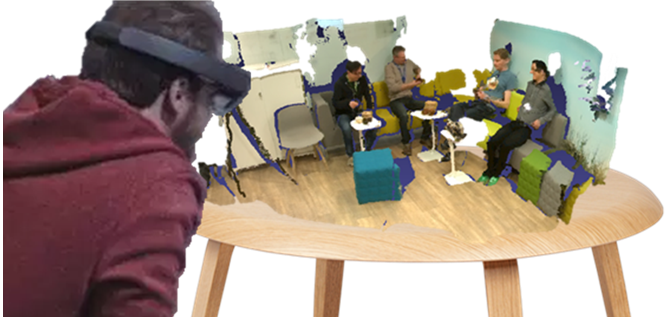
\includegraphics[scale=0.8] {tele_immersive.png}
	\caption[Tele-immersive experience enabled by point cloud compression.]{Tele-immersive experience enabled by point cloud compression.}
	\label{fig:Tele_immersive}
\end{figure}\\
Volumetric video represents 3D data in a way that the observer has freedom to navigate freely in the captured scene. Hence, such data has a high importance for virtual reality (VR), augmented reality (AR), or mixed reality (MR) applications, especially for providing six-degrees-of-freedom (6DOF) viewing capabilities. However, due to the large number of points which are generated to represent the scenery, limitations for storage and transmission over current network technology arise. Therefore, efficient compression algorithms are needed to help this technology to expand in all aspects. And these applications can be use in be in the construction business, agriculture and vegetation management, education and etc. Point clouds mainly use to represent the exterior surface of the object, but it can be utilized in medicine, for example, medical imaging to represent volumetric data.
\section{Objectives and Scope of the Thesis} \label{sec:Objectives_and_Scope_of_the_Thesis}
The conducted research study in this thesis was done in a collaboration of Nokia Technologies and Tampere University of Technology. This document describe technical details of improvement methods for the Nokia Technology submission \cite{NokiaResponseToCfP} to category two of the ISO/IEC JTC1/SC29/WG11 (MPEG) in response of Call for Proposals (CfP) for 3D point cloud compression \cite{CallforProposalsforPCC}. The aim of this proposed solution is to develop the needs of interactive, tele-immersive applications, such as VR, AR or MR with Six Degrees of Freedom (6DoF) capabilities. The proposed approach compress 3D video data by using 2D video standards. The main advantage of projection approach is its compatibility with current available 2D video coding standards. In addition, in terms of coding efficiency compare with reference technology it shows remarkable improvement which is proved by objective evaluation. Bitrate requirements is reduced by around 75\% for geometry and approximately 50\% for color attribute compression over the state-of-the-art compression technology. And from overall improvement almost one third is achieved by proposed algorithms in this thesis.\\
It is feasible to use video coding standards which are available for 2D video coding for point cloud compression, for instance Advanced Video Coding (H.264/AVC \cite{H.264_AVC}) or High Efficiency Video Coding (H.265/HEVC \cite{High_Efficiency_Video_Coding_HEVC}). The 2D video coding which is used for projection-based point cloud compression is scalability extension of HEVC (SHVC) reference software (SHM) \cite{HEVCScalabilityExtension}, in which one texture plane as a base layer and one geometry plane as an enhancement layer is used. It is also feasible to add more enhancement layer or using different video coding standard like 3D High Efficiency Video Coding (3D-HEVC \cite{3D_HEVC}). Since neither of these compression standards are designed for point cloud compression the demand for compression tool which is compatible with such content rise.\\
The projection-based point cloud compression significantly improved over the state-of-the-art method \cite{mekuria2017designTeleimersive} in terms of coding efficiency. However, this approach requires special attention on the sharp transitions at the projected object boundaries and sparsity in the 2D projections due to oversampling issues. Consequently, such areas create sub-optimal compression performance using the traditional 2D video compression technology.\\
The aim of this thesis is to provide solutions for the above-mentioned issues in order to improve the coding efficiency of the projection-based schemes. In this study, two processes have been proposed for this purpose. The first proposal targets improving the coding performance in the generated sharp edges of the projection-based method by applying a smoothing filter in the boundary areas. The edge smoothing operation intends to increase the correlation of samples in the boundary areas of the projected content in order to make it suitable for compression. Furthermore, the patch refinement is considered for filtering the sparsely projected point cloud data in projection plane for reducing sparsity and improving the compression performance. Figure \ref{fig:overall_process_of_projection_based} illustrates block diagram of overall process of the projection based point cloud compression.
\begin{figure} [t!]
	\centering
	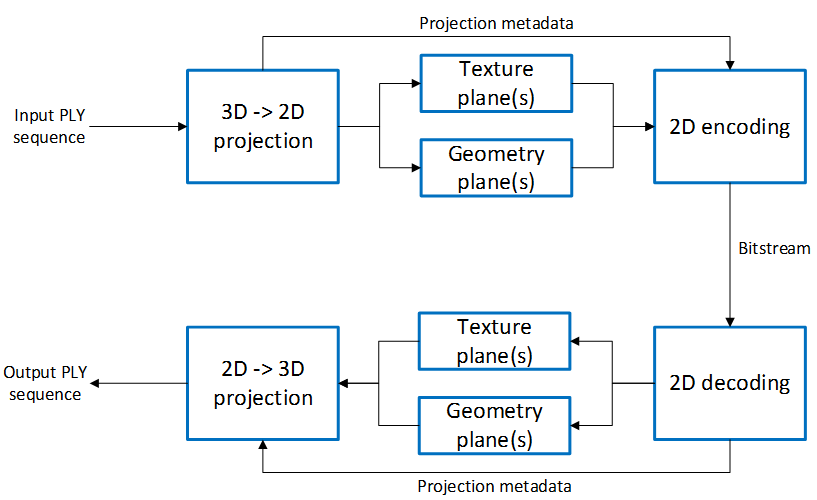
\includegraphics[scale=0.59] {overall_process_of_projection_based.png}
	\caption{The overall process of projection-based volumetric video coding.}
	\label{fig:overall_process_of_projection_based}
\end{figure}
\begin{itemize}
	\item \textbf{3D to 2D projection:} Projecting each individual point cloud of a sequence onto the selected 2D geometry. One 2D plane is allocated for texture projections and one for geometry.
	\item \textbf{2D encoding:}  The 2D planes are encoded with the current standard 2D video codecs (e.g SHM)
	\item \textbf{2D decoding:}  The encoded 2D planes are decoded with the current standard 2D video codecs.
	\item \textbf{3D to 2D projection:} The PLY can be reconstructed by using decoded planes (geometry and texture). In back projection process texture plane is used for color intensity value of point and the position of point is determined by corresponding geometry value.
\end{itemize}
\begin{figure}[!b]
	\centering
	\subfigure[]{%
		\label{fig:Original}%
		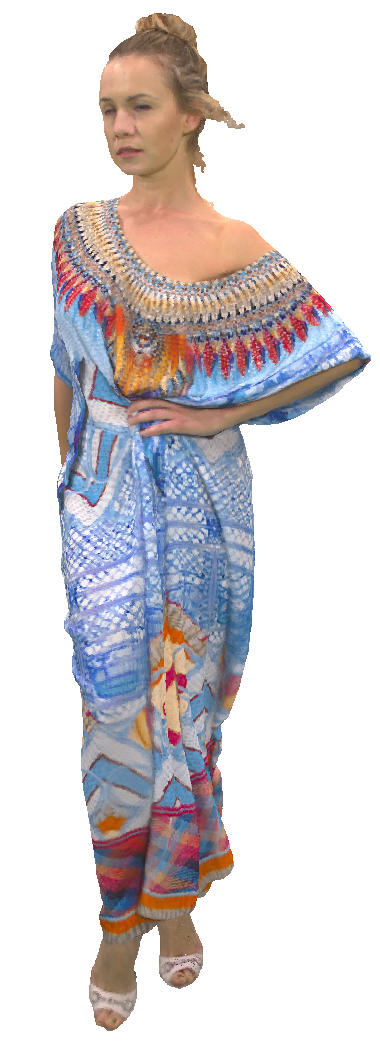
\includegraphics[scale=0.4]{Original.png}}%
	\subfigure[]{%
		\label{fig:projectionCodec}%
		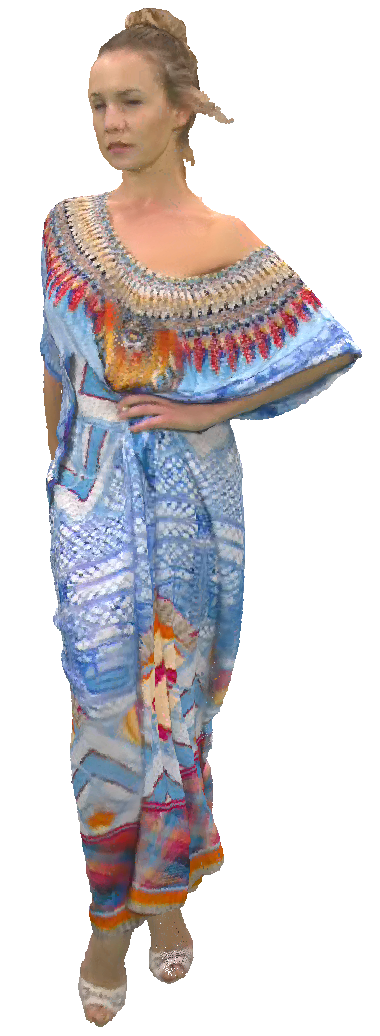
\includegraphics[scale=0.4]{projectionCodec.png}}%
	\subfigure[]{%
		\label{fig:referenceCodec}%
		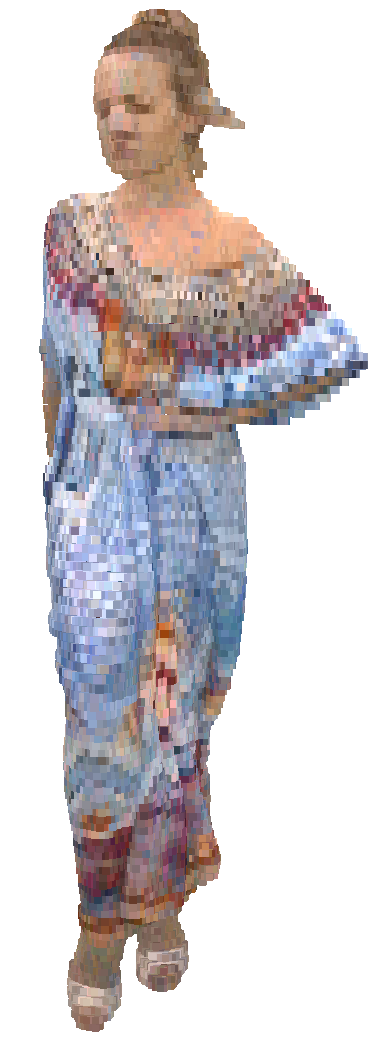
\includegraphics[scale=0.4]{referenceCodec.png}}%
	\caption{First frame of Longdress point cloud. Bounding box for point cloud (a), projection of the point cloud on 2D and assigning one image for texture and one for geometry (b)}
\end{figure}
\section{Thesis Outline}\label{sec:Thesis_Outline}
The rest of the thesis is organized as follows:
\begin{itemize}
	\item \textbf{Chapter 2:} Introducing different projection methods and functionality of projection based point cloud compression.
	\item \textbf{Chapter 3:} Discussing about the problems and  proposing methods to improved coding efficiency of projection based point cloud compression.
	\item \textbf{Chapter 4:} Analyzing the experimental results and related discussions.
	\item \textbf{Chapter 5:} Gives a conclusion and summary of the projection based point cloud and implemented algorithms.
\end{itemize}
\chapter{Projection based point cloud compression}\label{ch:projection_based_point_cloud_compression}
\section{Introduction}
There are variety of 3D to 2D projections exists and it is hardly possible to introduce one projection as the best projection for mapping since it is highly depended on the application. Whereas this work is a response to Call for Proposals (CfP) Category two of the ISO/IEC JTC1/SC29/WG11 (MPEG) for Point Cloud Compression, in which a test model are single 3D model. Thus, the approach and evaluation are provided in this context. Category two consist of scaning real moving moving people time instances. The target projection would cover the exterior part of the model.\\
In order to find the proper projection for the above-mentioned content the compression step which illustrates in Figure \ref{fig:overall_process_of_projection_based} has been removed to validate performance of the proposed projection method. Figure\ref{fig:test_projections} illustrate the general process of the projection test. In fact, in Figure \ref{fig:test_projections} the 2D encoder and decoder has been removed to test the functionality of projection. The functionality of projection is evaluated based on subjective and objective evaluation of the reconstructed point cloud. Here a desirable projection defines as a projection which covers more points, handles the occlusion of the reconstructed point cloud and also gain high Peak Signal to Noise Ratio(PSNR).\\
\begin{figure}
	\centering
	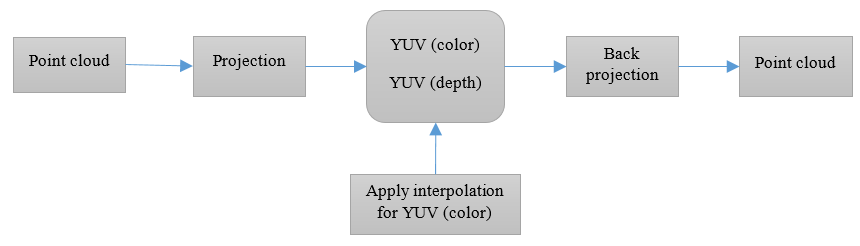
\includegraphics[scale=0.65] {test_projections.png}
	\caption{}
	\label{fig:test_projections}
\end{figure}

\section{Projection} \label{sec:Projection}
Here projection defines as a transformation which performs translation from 3D Cartesian coordinate to 2D coordinate. Different approaches for projection have been proposed and tested. In the following all projection which examined for this study are presented.\\
Before performing any projection, in order to project samples of point cloud in 2D space it is essential to analyze and initialize basic parameters. One of the most important one is bounding box which is based on the attribute (minimum and maximum) of point cloud. In geometry, the bounding box is the smallest or minimum box which encloses all set of points in N dimension where in the 3D space the bounding box is a cuboid shape. Figure \ref{fig:bounding_box} shows a bounding box for \textit{Longdress} point cloud in which all samples are surrounded by bounding box. Another substantial parameter is primary axis which is defined as longest axis of bounding box. The best primary axis for the test data which are used for this experiment is Y-axis.\\
A 3D video object, e.g represented as a dynamic sequence of point clouds, is projected onto simple geometries. For each projection process two 2D image planes are assigned, one for color attribute (texture image) and one for 3D depth (geometry image). Figure \ref{fig:texture_geometry} shows the texture and geometry image for one frame of \textit{Longdress} sequence projected onto plane projection.\\
\begin{figure*}[!tbp]
	\centering
	\subfigure[]{%
		\label{fig:bounding_box}%
		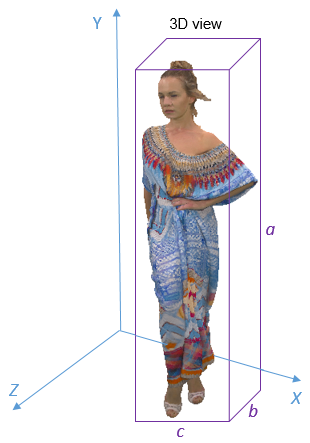
\includegraphics[scale=0.6]{bounding_box.png}}%
	\qquad
	\subfigure[]{%
		\label{fig:texture_geometry}%
		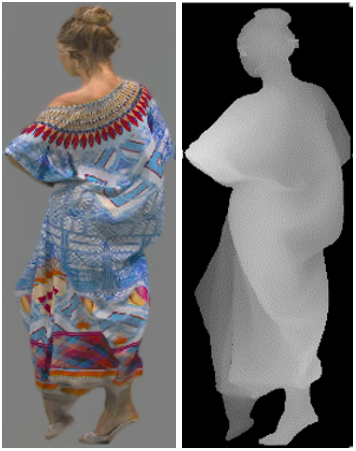
\includegraphics[scale=0.6]{texture_geometry.png}}%
		\label{fig:bbox_texture_geometry}%
	\caption{First frame of Longdress point cloud. Bounding box for point cloud (a), projection of the point cloud on 2D and assigning one image for texture and one for geometry (b)}
\end{figure*}\\
The length of the space diagonal is calculated by:\\

\begin{equation} \label{eq:diagonal_of_bbox}
\begin{aligned}
d = \sqrt{a^{2}+b^{2}+c^{2}}
\end{aligned}
\end{equation}

The position of 3D points after projection in 2D space is derived from :

\begin{subequations}
	\begin{align}
	length_{x} = max_{x}-min_{x}\\
	length_{y} = max_{y}-min_{y}\\
	length_{z} = max_{z}-min_{z}
	\end{align}
\end{subequations}
\begin{subequations}
	\begin{align}
	position_{x} = \lfloor{\dfrac{x-x_{min}}{x_{max}-x_{min}}*length_{x}}\rfloor +1\\
	position_{y} = \lfloor{\dfrac{y-y_{min}}{y_{max}-y_{min}}*length_{y}}\rfloor +1\\
	position_{z} = \lfloor{\dfrac{z-z_{min}}{z_{max}-z_{min}}*length_{z}}\rfloor +1
	\end{align}
\end{subequations}
In which length of cube edges is calculated by subtracting minimum value of coordinate from maximum value and it should be multiple of 8 (nemidoanm Ask Ramin).

After projecting 3D  model to 2D images. Due to the possible sparsity of the point cloud data, the 2D projections may contain points without any value assigned.Such points create inefficiencies in the compression process and affect the projection-based scheme sub-optimal. In order to solve this issue, interpolation is applied to calculate the intensity value for missing pixel between known-value pixels. In the texture plane, these null value pixels are interpolated in the horizontal direction by using a linear interpolation method. Linear interpolation:
\begin{equation} \label{eq:diagonal_of_bbox}
\begin{aligned}
f(n+i) = \frac{(d - i)*f(n)+i*f(n+d)}{d} ,\quad  0<i<d
\end{aligned}
\end{equation}
In which f(n) and f(n+d) are knwon values and d is distance between two known value. By using such inpainting operation, the missing values will be assigned to a particular color value based on their neighboring color information. The higher weights are assigned to closer color intensity value which are unknown. The inpainting process is only applied to the texture plane and not to the geometry plane, as the geometry plane is essential for the reconstructing the 3D volumetric data. Occupancy map which is derived from geometry plane is an image in which occupied pixels are assigned to one and empty ones are zero, so only pixels which their corresponding occupancy map is one are reproject back to 3D space. If inpainting also applied on the geometry plane, the reconstructed 3D data would include many invalid 3D points, unless generating occupancy map before interpolating geometry plane. Figure \ref{fig:sparse_reddress} shows the texture plane of \textit{Redandblack} sequence as it can be seen some null values in texture plane are shown as black and Figure \ref{fig:inpainted_sparse_projection} depicts the applying linear interpolation in horizontal direction. The interpolated values will not reconstruct in the back projection from 2D to 3D since the occupancy map for those interpolated values are zero.
\begin{figure*}[!tbp]
	\centering
	\subfigure[]{%
		\label{fig:sparse_projection}%
		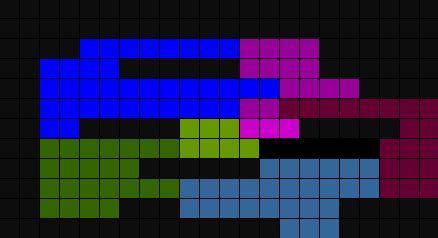
\includegraphics[scale=0.5]{sparse_projection.png}}%
	\qquad
	\subfigure[]{%
		\label{fig:inpainted_sparse_projection}%
		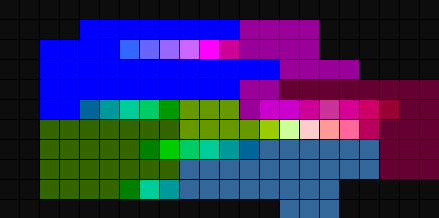
\includegraphics[scale=0.55]{inpainted_sparse_projection.png}}%
	\caption{(a)sparse projection of model (b) inpainted sparse projection by linear interpolation.the colors are exaggerated for illustrative purposes.}
\end{figure*}

\begin{figure*}[!tbp]
	\centering
	\subfigure[]{%
		\label{fig:sparse_reddress}%
		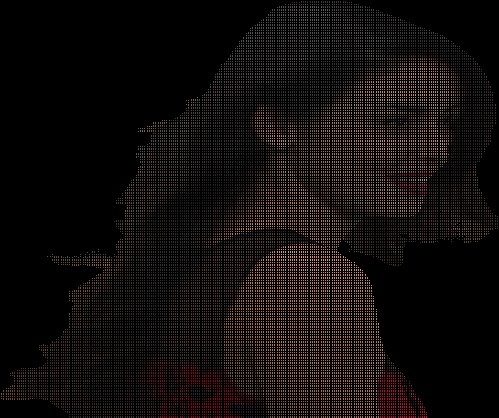
\includegraphics[scale=0.4]{sparse_reddress.png}}%
	\qquad
	\subfigure[]{%
		\label{fig:inpanted_reddress}%
		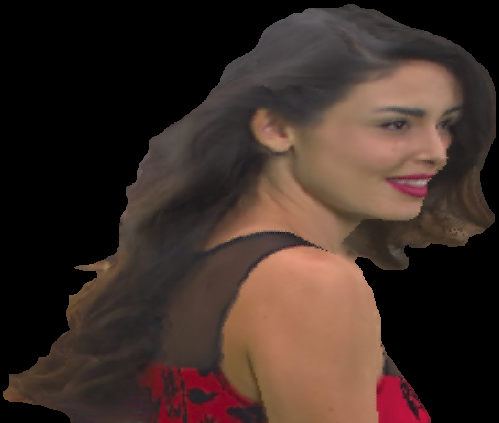
\includegraphics[scale=0.4]{inpanted_reddress.png}}%
	\caption{(a)sparse projection of model (b) small holes are filled by applying interpolation.}
\end{figure*}

\subsection{Sphere}\label{sec:sphere_projection}
This transformation turns the location of points in Cartesian space to spherical coordinates.
\begin{figure}[t!]
 	\centering
	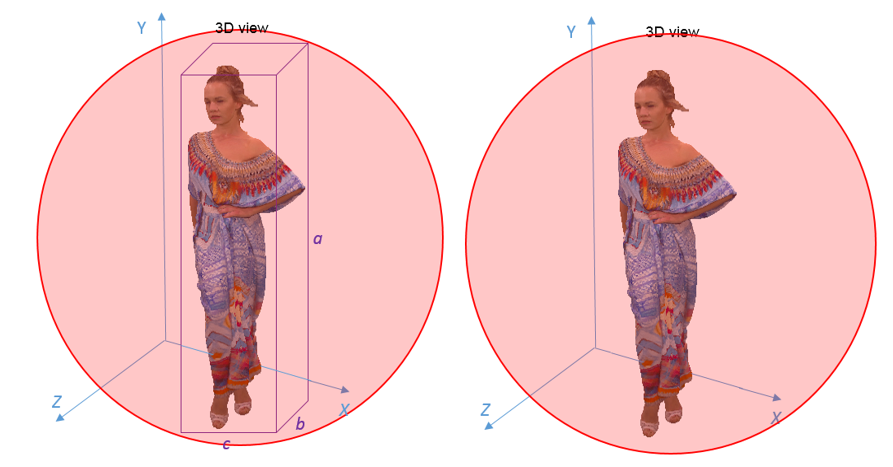
\includegraphics[scale=0.6] {sphere_projection.png}
	\caption{}
	\label{fig:sphere_projection}
\end{figure}
Radios (R) of the sphere is calculated by multiplying the arbitrary number larger than one (ex.1.2) with the length of diagonal bounding box.\\
\begin{subequations}
	\begin{align}
	R_{sp} = d*1.2\\
	X_{sp} = \arccos \dfrac{X}{R}*d\\
	Y_{sp} = \arccos \dfrac{X}{R}*d\\
	Z_{sp} = \arccos \dfrac{X}{R}*d
	\end{align}
\end{subequations}
The conversion from three-dimensional Cartesian coordinates into azimuth and elevation for equirectangular mapping is derived:\\
\begin{subequations}
	\begin{align}
	H = \sqrt{X_{sp}^{2}+Y_{sp}^{2}}\\
	r = \arccos \dfrac{X}{R}*d\\
	azimuth = \atantwo(Z_{sp},H)\\
	elevation = \atantwo(Y_{sp},X_{sp}) 
	\end{align}
\end{subequations}
\begin{figure}[t!]
	\centering
	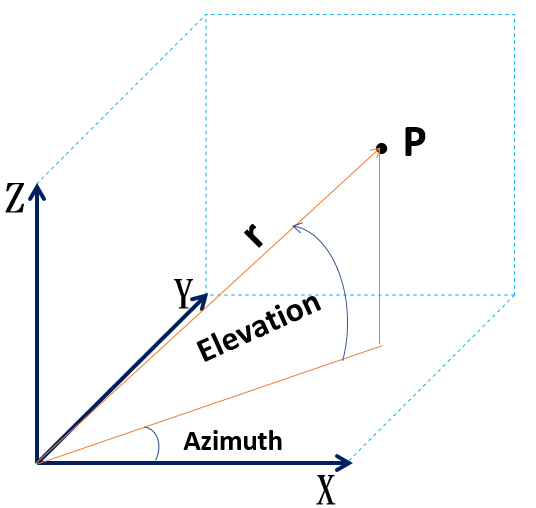
\includegraphics[scale=0.5] {cartesian.png}
	\caption{}
	\label{fig:cartesian}
\end{figure}
Where r is radius and distance from the origin to a point where both azimuth and elevation are in radian. Azimuth is the counterclockwise angle in the x-y plane from the positive x-axis. The elevation is angle in radians from the x-y plane. 
Pixel coordinates for the equirectangular picture is calculated by:
\begin{subequations}
	\begin{align}
	x_{pos} = \lfloor{\dfrac{azimuth + \pi}{\dfrac{2\pi}{width}}}\rfloor+1\\
	y_{pos} = \lfloor{\dfrac{elevation+\dfrac{\pi}{2}}{\dfrac{2\pi}{width}}}\rfloor+1
	\end{align}
\end{subequations}
The problem with sphere projection is that it does not preserve all points in 3D models which are not round .(nemidoanm Explain why?)
image. Figure \ref{fig:shpere_projection_rec_egyption} and \ref{fig:shpere_projection_rec_longdress} shows reconstructed result of two point clouds with same projection, as it can be seen it highly depends on the overall structure of the original content.\\
\begin{figure}%
	\centering
	\subfigure[]{%
		\label{fig:shpere_projection_original_egyption}%
		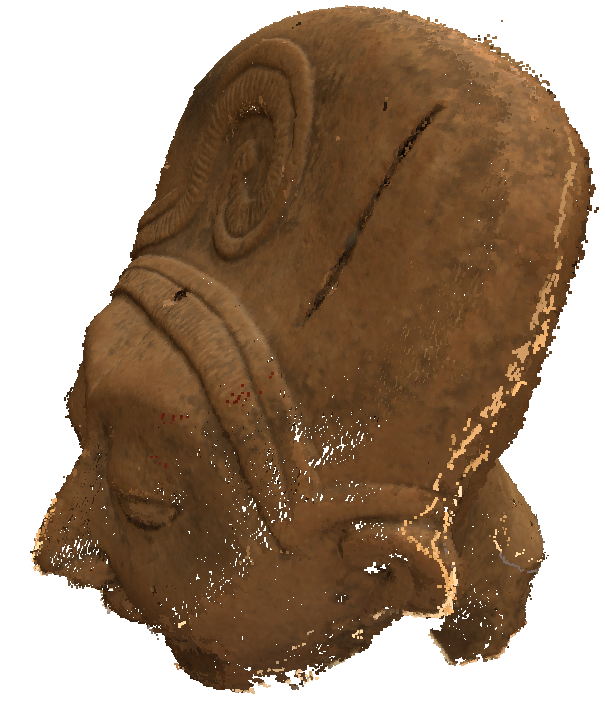
\includegraphics[scale=0.3]{shpere_projection_original_egyption.png}}%
	\subfigure[]{%
		\label{fig:shpere_projection_rec_egyption}%
		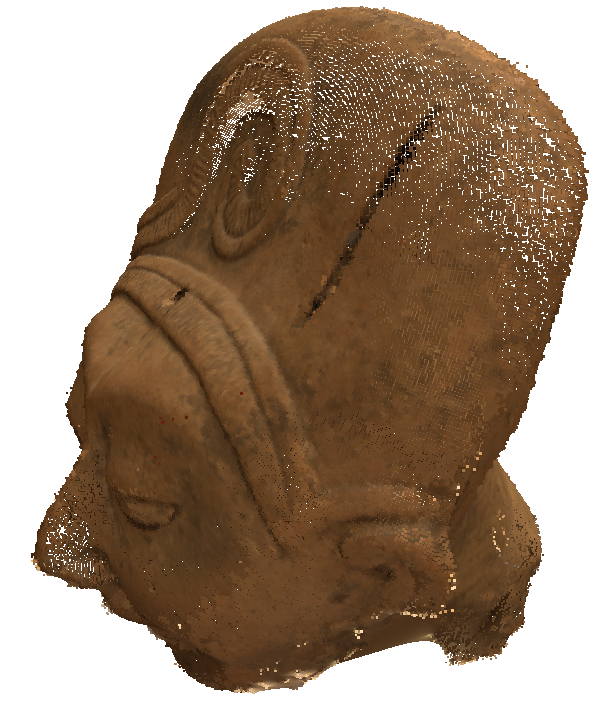
\includegraphics[scale=0.3]{shpere_projection_rec_egyption.png}}%
	\subfigure[]{%
		\label{fig:shpere_projection_original_longdress}%
		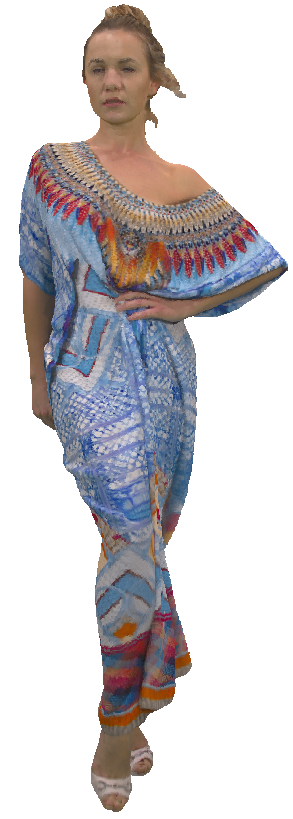
\includegraphics[scale=0.4]{shpere_projection_original_longdress.png}}%
	\subfigure[]{%
		\label{fig:shpere_projection_rec_longdress}%
		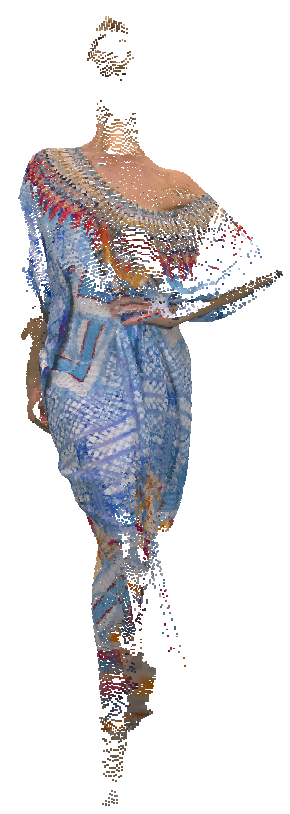
\includegraphics[scale=0.4]{shpere_projection_rec_longdress.png}}%
	\label{Comparison_result_Cylinder_projection}
	\caption{(a) Original \textit{Egyption} point cloud (b) reconstructed point cloud in sphere projection (c) Original \textit{Longdress} point cloud (d) reconstructed point cloud in sphere projection}
\end{figure}
\subsection{Cylinder}\label{sec:cylinder_projection}
The second kind of projection which examined is cylinder projection. Similar to sphere projection it project points into the corresponding coordinates which is follow this relation:\\
\begin{subequations}
	\begin{align}
		r = \sqrt{X^{2}+Z^{2}}\\
		R_{cy} = r*1.2\\
		X_{SP} = \arccos (\frac{X}{r})\\
		Y_{SP} = 1\\
		Z_{SP} = \arccos (\frac{Z}{r})
	\end{align}
\end{subequations}
In this projection firstly points project onto cylinder position, then unfold cylinder and use it as 2D image.\\
\begin{figure}
	\centering 
	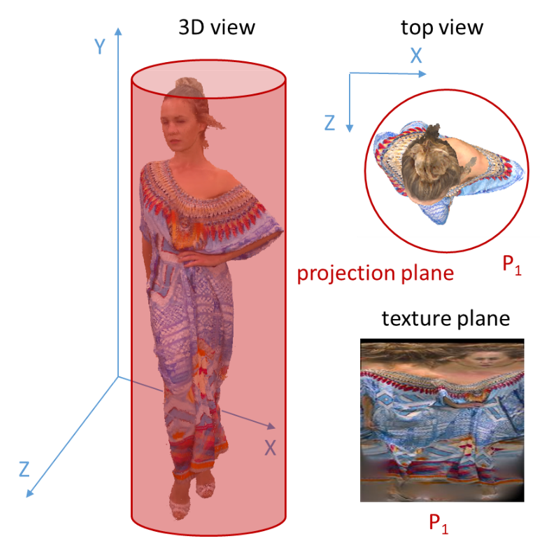
\includegraphics[scale=0.7] {cylinder_projection.png}
	\label{fig:cylinder_projection}
	\caption{}
\end{figure}
\subsection{Cube}\label{sec:cube_projection}
This projection is used for projecting points in 3D space onto 4 sides of the cube. In fact, the goal of this projection is to see the 3D object from 4 different perspectives of the cube. For each side, the decision is made based on the distance of the point to plane. Since there is a possibility to map more than one point from 3D space onto the same 2D coordinate, depth buffering is applied to handle this problem. Depth buffering stores the distance from the closest point to the 2D plane. Firstly, the projections are done on two opposite sides of the plane. For instance, if there are four planes of projection namely right, front, left and back. Right and left planes which are opposite sides of the cube process (project and back project) simultaneously and same for front and back. Before projecting one point in the texture plane first it should be investigate whether the point which intends to project on texture plain is null or it is occupied in advance.\\
In the case that more than one 3D point is mapped on the same 2D coordinates Z-buffer is used to compare the distance of the old point and new point to the plane. And the point which has the smaller distance with plane will be store in depth buffer and consequently its color attribute.For the later one since the location of the current point is similar the occupied point comparing the distance is the solution to project the closest points to the 2D plain and store the distance of the corresponding point in the Z-buffer and color channel separately store it in texture plain. Information about the lost points for further processing and comparison can be stored.\\
\begin{figure*}[!tbp]
	\centering 
	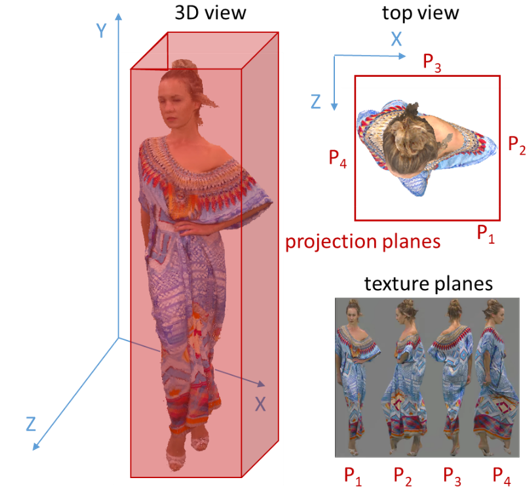
\includegraphics[scale=0.7] {planer_rotation_projection.png}
	\caption{3D to 2D projection onto four rectangular planes and Y is primary axis}
	\label{fig:planer_rotation_projection}
\end{figure*}
\begin{figure*}[!tbp]
	\centering
	\subfigure[]{%
		\label{fig:Texture_projection}%
		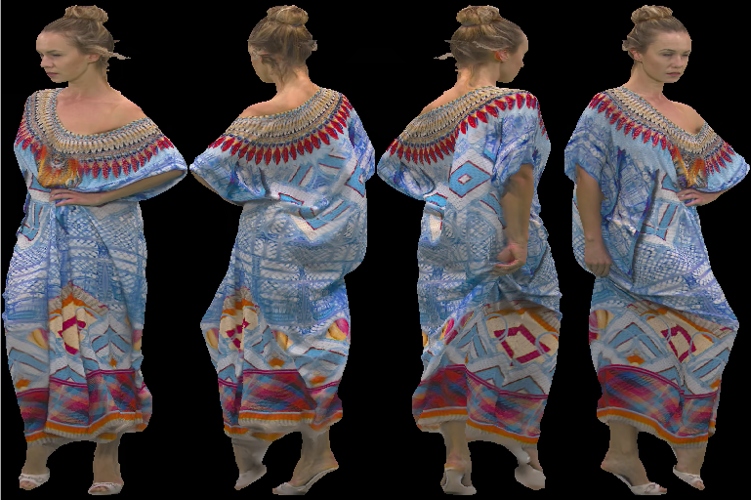
\includegraphics[scale=0.35]{4rot.png}}%
	\qquad
	\subfigure[]{%
		\label{fig:Geometry_projection}%
		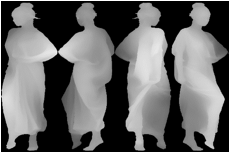
\includegraphics[scale=1.16]{depth_4rot.png}}%
	\caption{(a) Texture and (b) geometry projection images examples for \textit{Longdress} sequence.}
\end{figure*}
\subsection{Planer rotation}\label{sec:planer_rotation}
This projection is similar to projecting on cube ,but all 4 projections (front, left, back and front) are stitched together to make one texture image and one geometry. Figure \ref{fig:planer_rotation_projection} depicts one example projection with four planes and 90-degree rotation between each plane where the starting plane is ${P_{1}}$ and aligned to X axis. In this example Y is primary axis, since between the value ranges of X,Y, and Z, with Y>X>Z, Y axis has wider ranges of values and selected as primary axis and X as an secondary axis. This projection is the base of further implementation for projection-based point cloud compression and for this study, a projection onto series of rectangular planes is chosen. Occlusion can improved by increasing the number of projection as depicts in Figure \ref{fig:make_8_rot_dicriptionOfLaw_nemidoanm}. The offset after the first four rotations is applied to help better coverage of the 3D volume and reducing occlusions.
\subsection{Sequential Decimation}\label{sec:sequential_decimation_projection}
As illustrated in figure \ref{fig:make_8_rot_dicriptionOfLaw_nemidoanm} there is a considerable similarities between the first four orations and the last four rotations, thus sequential decimation is introduced. This extension adds more projection of surfaces at different rotations to cover the exterior side of 3D object more coherently. Yet, adding projections does not necessarily cover all the areas. Figure \ref{fig:sequential_decimation_after_each_projection} depicts the concept of sequential decimation, as shown points which are projected successfully removed from point cloud, therefore the last projection is more spare in comparison the first one.\\
Figure \ref{fig:sequential_decimation_a} represents an example of sequential decimation with 4 primary rotations and 4 additional rotations. As it can be observed, those points which are successfully projected in the first 4 rotations are removed, then the rotation plane is shifted by 45 degrees to cover points which do not have chance to project in the earlier projections. These additional rotations create sparse data in the projection plane which are not favorable for standard 2D video codecs.\\
\begin{figure*}[!tbp]
	\centering 
	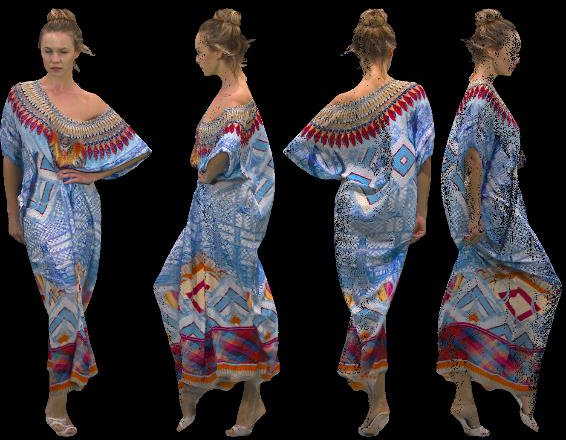
\includegraphics[scale=1] {Effect_of_sequential_decimation_after_each_projection.png}
	\caption{Effect of sequential decimation after each projection}
	\label{fig:sequential_decimation_after_each_projection}
\end{figure*}
\begin{figure}
	\centering 
	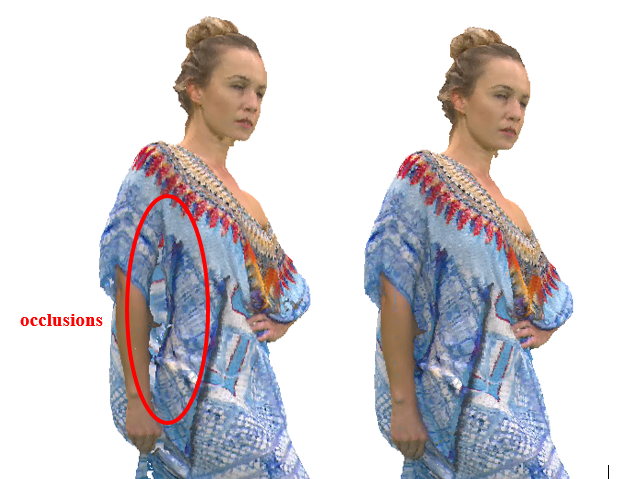
\includegraphics[scale=2.5] {Improved_occlusion_handling_provided_sequential_decimation.png}
	\caption{Sequential decimation improves the occlusion handling (left)}
	\label{fig:Improved_occlusion_handling_provided_sequential_decimation}
\end{figure} 
\chapter{Proposed Methods}\label{sec:proposed_methods}
As described in Section \ref{sec:sequential_decimation_projection} the projection-based approach provides significant compression performance improvements over the state-of-the-art. However, the projected 2D data has sharp boundaries, which introduce crucial issues when using conventional block-based DCT video coding schemes. In the object boundaries, some blocks may contain partial data from the projected point cloud content and partially from the image plane background. In the encoding process, these are represented as high-frequency DCT components, which result in extra bitrate and decrease reconstruction quality.\\
Also, due to the possible sparsity of the point cloud data, the 2D projections may contain points without any value assigned. Such points create inefficiencies in the compression process and affect the projection-based scheme sub-optimal. In order to solve this issue, we use inpainting for calculating the missing pixel values between known-value pixels. In the texture plane, these null value pixels are interpolated in the horizontal direction by using a linear interpolation method. By using such inpainting operation, the missing values will be assigned to a particular color value based on their neighboring color information. The inpainting process is only applied to the texture plane and not to the geometry plane, as the geometry plane is essential for the reconstructing the 3D volumetric data. Only pixel with a valid geometry value are reprojected back into 3D space. If inpainting would also be applied on the geometry plane, the reconstructed 3D data would include many invalid 3D points.
\section{Edge Smoothing}
\label{ssec:edge_smoothing}
First, the unoccupied projection planes (i.e., geometry and texture) are initialized with zero values for each pixel. Then, the 3D data is projected onto the corresponding 2D planes. Prior to the edge smoothing operation, the background samples are replaced with gray values (i.e., equal to 128 in 8 Bit YUV color space). Then, edge smoothing is applied to the projected point cloud boundaries. This technique includes applying averaging filters in horizontal and vertical direction successively. For this purpose, the averaging filter of equation (\ref{eq:1}) is used. In this formula, N is the filter kernel size and $X_{i,j}$ is the pixel value at (i,j) location inside the filter kernel. In our experiments, the kernel size of 7 provided the best results.
\begin{equation} \label{eq:1}
\begin{aligned}
P = \dfrac{\sum_{i=0}^{N-1} \sum_{j=0}^{N-1}X_{i,j}}{N^2},
\end{aligned}
\end{equation}
Figure \ref{fig:averaging} illustrates an example of applying the proposed edge smoothing filter in horizontal direction. The blue part indicates a portion of the projected point cloud. The purple, pink and green kernels show the filter kernels that are applied in horizontal direction. The smoothing process stops at projected data boundaries. Moreover, it does not affect the pixel values inside the projection areas.

By employing this algorithm, in both horizontal and vertical directions, the sharp intensity transitions in the boundaries between the point cloud content and background is reduced. And reducing this contrast, results in a coherent and smooth transition between the projected point cloud data and the image plane background. Therefore, the decorrelation process in the compression operation can take place properly and the bitrate would decrease significantly.
\begin{figure}[t!]
	\centering 
		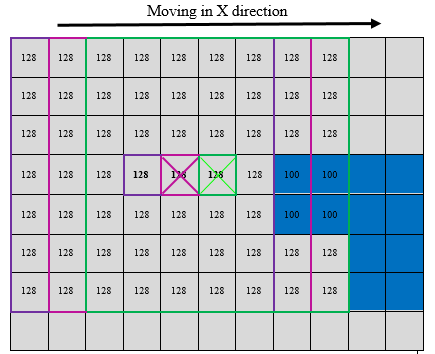
\includegraphics[scale=0.7]{Average}
		\caption{Employing edge smoothing in horizontal direction.}
		\label{fig:averaging}
\end{figure}

\begin{landscape}
	\begin{figure}[t!]
		\begin{center}
			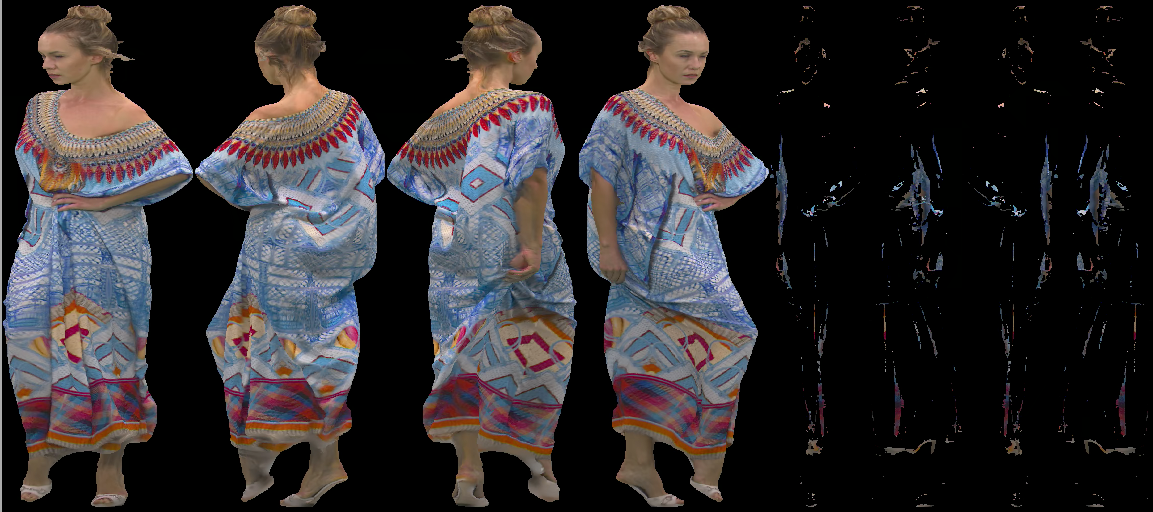
\includegraphics[scale=0.55] {original_8rot.png}
			\textsf{}\\
			\textsf{}\\
			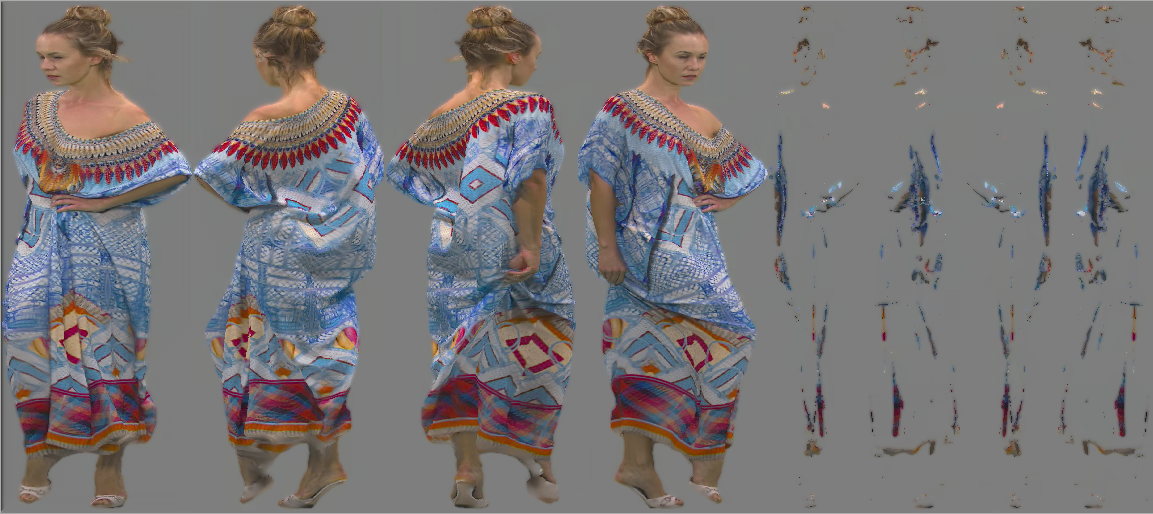
\includegraphics[scale=0.55] {gray_average_8rot.png}
		\end{center}
		\caption{Texture plane for decimation rotation (top) edge-Smoothing applied for projected 3D data (bottom)}
		\label{fig:longdress_averaging}
	\end{figure}
\end{landscape}

\section{Patch Refinement}
\label{ssec:refinement}
As it was mentioned in Section \ref{sec:sequential_decimation_projection}, sequential decimation provides additional projections to cover the points which are not initially projected to the projection plane. As a result, their projections have a sparse distribution, as it can be seen in Figure \ref{fig:longdress_averaging} (the last 4 projections). Such sparsity is not desirable in image/video coding algorithms and increases the bitrate significantly.

In order to decrease the effect of this sparse content, a method is studied in this section that uses a filtering operation for reducing the number of sparse content in a way that can improve the compression performance and has negligible impact on the quality of the decoded point cloud data.

For this purpose, after the interpolation and edge smoothing processes, a binary occupancy mask is extracted from the output texture plane for processing such small patches. The binary occupancy mask is a mask which indicates occupied pixels in texture plane. The patch refinement operation includes a process of removing the samples in a certain area of the sparse data that have less connection to the neighboring samples than a per-defined threshold (i.e., based on number of samples). This process is illustrated in Figure \ref{fig:Patch_refinement}.
A it can be seen from the Figure, a 3$\times$3 filter is selected for this analysis. The filter kernel is applied to the sparse sampling area and detects whether the central point of the kernel has connections to at least three samples inside the kernel. Otherwise, the value of the point will be replaced by the background value in both texture and geometry images. In another words, The more connection a certain point has with its neighborhood samples, the more probable to preserve the point. In the example of Figure \ref{fig:Patch_refinement}, the center point of the red kernel is connected to only one point, so this point will be removed. Whereas, for the green kernel the center value is connected to 4 neighbors, so no change will occur. 

As a result of the re-filtering operation in patch refinement, the discontinuity of the samples in the sparse area is reduced and consequently the required bitrate will decrease significantly.


\begin{figure}[t!]
	\centering 
	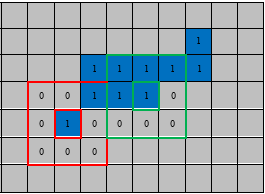
\includegraphics[scale=0.9]{Removing_smallPoints}
	\caption{An example of applying patch refinement.}
	\label{fig:Patch_refinement}
\end{figure}

\begin{landscape}
	\begin{figure}[t!]
		\begin{center}
			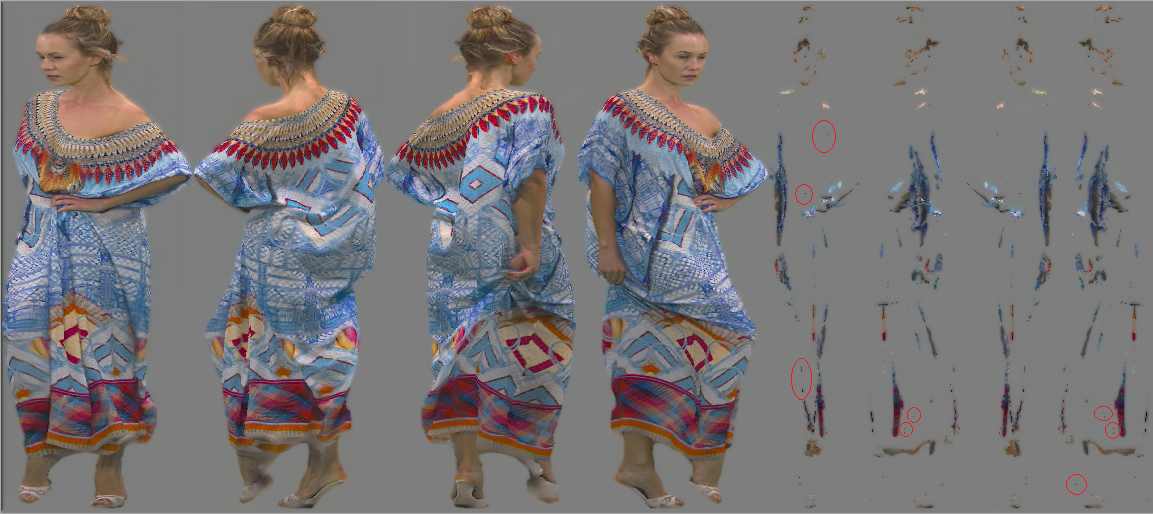
\includegraphics[scale=0.55] {gray_blur_8rot_problem.png}
			\textsf{}\\
			\textsf{}\\
			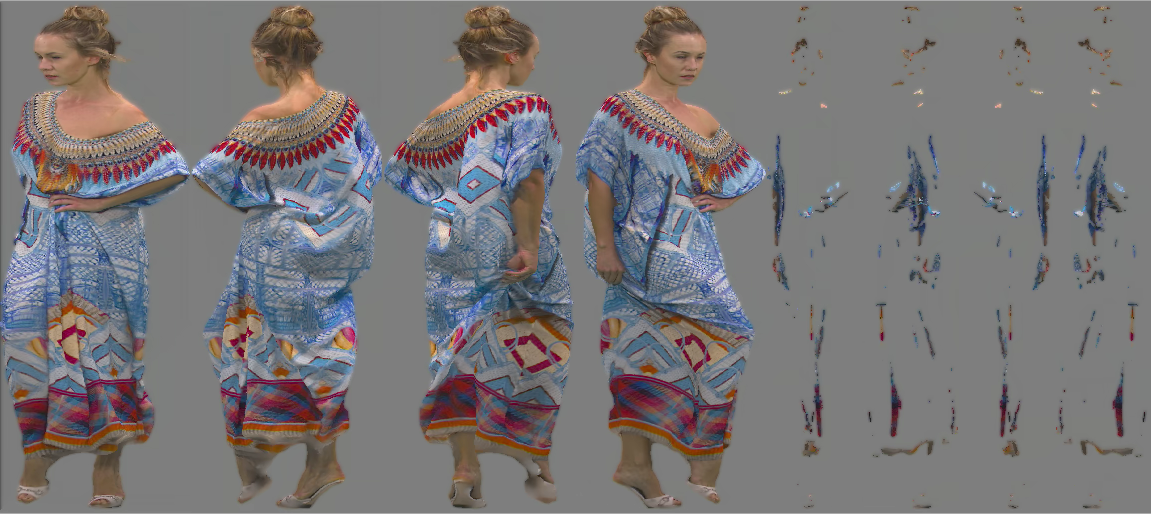
\includegraphics[scale=0.55] {gray_blur_8rot_patchref.png}
		\end{center}
		\caption{Texture plane for decimation rotation after applying edge-Smoothing(top) patch refinement is applied for projected 3D data (bottom)}
		\label{fig:longdress_patch_refinement}
	\end{figure}
\end{landscape}

\chapter{Experimental Results} 
This chapter presents the experimental condition, results and analysis of the implemented method which is proposed in chapter \ref{sec:proposed_methods}.\\
The proposed algorithms are implemented in the HM version 16.6, the HEVC reference software \cite{HEVCScalabilityExtension} and test condition done under 5 different quantization parameters (QP). Results were provided for dynamic objects test (category two), and testing condition is for all intra and random access. The performance of proposed algorithms was analyzed with the well-known Bj�ntegaard delta bitrate (BDBR) metric [16], in which the negative values represent the bitrate reduction in the same peak signal-to-noise ratio (PSNR) and the positive values indicate the bitrate loss for the same PSNR value.\\

\section{Point Cloud Data} \label{sequences}

In the simulations 4 video sequences which are provided by 8i \cite{8i_Voxelized_Full_Bodies} are used to evaluate the performance of the proposed methods. Table\ref{Video_Seq} shows a list of the 3D point cloud test material dataset and their specifications.\\

\begin{table}
	\centering
	\caption{Video Sequences of dynamic objects test Category two are used in this experiment}
	\label{Video_Seq}
	\scalebox{0.80}{
		\begin{tabular}{|c|c|c|c|c|}
			\hline
			Test material dataset filename & Number of frames & Pts & Geometry
			Precision & Attributes \\
			\hline
			8i VFB  Loot 		  & 300 &  ~782,000   & 10 bit & R,G,B\\
			8i VFB  RedandBlack   & 300 &  ~700,000   & 10 bit & R,G,B\\
			8i VFB  Soldier		  & 300 &  ~1,500,000 & 10 bit & R,G,B\\
			8i VFB  Longdress 	  & 300 &  ~800,000   & 10 bit & R,G,B\\
			\hline
	\end{tabular}}
\end{table}	

\section{Objective Evaluation Criteria and Metrics}\label{evaluation_criteria}

The evaluation of 2D video coding of volumetric data was performed under MPEG CfP for point cloud compression condition. For more details, please refer to the CfP document \cite{CallforProposalsforPCC} and its corrigenda \cite{Corrigenda}. The proposed methods have been implemented within the scalable extension of the HEVC standard (SHVC) SHM reference software version 12.2  \cite{HEVCScalabilityExtension}. The performance was analyzed for five different bitrate targets in the range from 3 to 43 Mbit/s in random access (RA) configuration. Four point cloud sequences were evaluated, each consisting of 300 frames.

Two different metrics were calculated to assess the geometry distortion. The first metric is a point-to-point quality assessment (referred to as D1 metric) which computes the mean square error (MSE) between the reconstructed point and its closest point in the original point cloud. The second metric assesses the point to the plane error (referred to as D2 metric). D2 calculates the MSE between the reconstructed point and the original point cloud surface \cite{tian2017geometricDistortionMetrics}. The color distortion is computed on a point-to-point level in YUV domain. The performances were analyzed based on the well-known Bj{\o}ntegaard Delta Bitrate (BDBR) criterion \cite{TourapisBDRate}, in which the negative values indicate the bitrate reduction in the same peak signal-to-noise ratio (PSNR) quality. Similarly, the positive values represent how much the bitrate is increased in the same quality level.

\subsection {Geometric Distortions}
The point cloud is define as a set of points without specific order in 3D space and all points have the same number of attributes. The most crucial attributes are geometry location (x,y,z) and color components (r,g,b) or (y,u,v). Let assume \textbf{A} as an original point cloud and \textbf{B} as a decoded compressed point cloud. \textbf{A} is reference for computing the quality of a \textbf{B} which is a degraded version of \textbf{A} and consist of N points. Where the number of points in original and degraded one are not necessarily equal. Compression error which is point cloud \textbf{B} relative to the reference point cloud \textbf{A} is denoted by $e_{A,B}$. Nearest neighbor is used to identify the correspondence between in \textbf{B} and \textbf{A}. n this case in order to reduce the computational complexity KD-tree search is utilized. If points in \textbf{B} is denoted by $b_{j}$ the corresponding point in \textbf{A} is identified by KD-tree to perform nearest neighbor search and denoted by $a_{j}$. In the Figure \ref{fig:Illustration_D1_and_D2} the black point is collected from point cloud \textbf{B} and the red point is the corresponding point of $b_{j}$ in point cloud \textbf{A}.\\

\textbf{Computing D1} \\
After identifying the point of \textbf{B} in uncompressed point cloud \textbf{A}. An error vector E(\textit{i,j}) is calculated by connecting \textbf{A} to the point \textbf{B}. The length of error vector E(\textit{i,j}) is called point-to-point error:\\
\begin{equation}
	\centering
	e_{A,B}^{D1}(i) = ||{E(i,j)}||^{2}_{2}
	\label{eq:one_point_to_point}
\end{equation}
Based on the definition of point-to-point distance for one point in \ref{eq:one_point_to_point}, for calculating point to point error (D1) for all the points in \textbf{B}, with $N_{B}$ number of points, is defined as:\\
\begin{equation}
	\centering
	e_{A,B}^{D1} = \dfrac{1}{N_{B}} \sum_{\forall b_{i} \in B} {e_{A,B}^{D1} (i)}
\end{equation}
\begin{figure}[t!]
	\centering 
	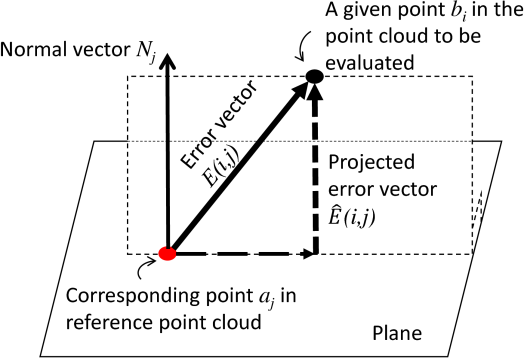
\includegraphics[scale=1.3]{Illustration_D1_and_D2.png}
	\caption{Illustration of point-to-point distance (D1) and point-to-plane distance (D2) \cite{CallforProposalsforPCC}}
	\label{fig:Illustration_D1_and_D2}
\end{figure}\\
\textbf{Computing D2}\\
Projection of the error vector E(\textit{i,j}) along the normal direction $N_{j}$ result in new error vector $\hat{E}(\textit{i,j})$  which is parallel with normal. D2 calculates the Mean squared error (MSE) between a reconstructed point and the original point cloud surface \cite{tian2017geometricDistortionMetrics}. The point-to-plane error is computed as:\\
\begin{equation}
	\centering
	e_{A,B}^{D2} = ||\hat{E(i,j)}||^{2}_{2} = (E(i,j).N_{j})^{2}
\end{equation}
Similarly the point-to-plane error (D2) for all of points is calculated by:
\begin{equation}
	\centering
	e_{A,B}^{D2} = \dfrac{1}{N_{B}} \sum_{\forall b_{i} \in B} {e_{A,B}^{D2} (i)}
\end{equation}
\textbf{Geometry PSNR Calculation}\\
The PSNR value for geometry attribute is computed as:
\begin{equation}
	\centering
	PSNR = 10\log_{10} (\dfrac{3p^{2}}{MSE}) 
\end{equation}
For each reference point cloud as specified in Table [nemidoanm] p is defined as the peak constant value. And MSE is the mean squared error of one of the errors (point-to-point (D1) or point-to-plane (D2)) which introduced before.\\

\textbf{Color PSNR Calculation}\\
The PSNR value for color attribute is computed as:\\
\begin{equation}
	\centering
	PSNR = 10\log_{10} (\dfrac{p^{2}}{MSE}) 
\end{equation}
For color attributes, the MSE for each of the three color components is calculated. Color distortion is performed in YUV color space, since YUV color space is closer to human perception. Therefore, if the color space of the point cloud is other than YUV color conversion is performed. A symmetric computation of the distortion is calculated, with the same method which done for geometric distortions. The maximum distortion between the two execution is selected as the final distortion. For PSNR calculation of color the peak vale p is 255, hence the bit depth for test data is 8 bits per point.\\

\section{Results for applying Edge-smoothing and patch refinement} \label{Applying_Edgesmoothing_and_patchrefinement_results}
This section presents the results of implemented proposed algorithms for 2D compression of point cloud data.\\


\section{Applying Edge-smoothing}
\textbf{All Intra Coding Results}\\
\begin{table}
	\centering
	\caption{BD-Rate (\%) and BD-PSNR [dB] performances for Intra-frame and applying Edge-smoothing}
	\label{Intra_frame_Edgesmoothing}
	\scalebox{0.80}{
		\begin{tabular}{|c|c|c|c|c|c|c|c|c|c|c|}
			\hline
			\multirow{2}{*}{Sequence} & \multicolumn{5}{c|}{BD-Rate (\%)} & \multicolumn{5}{c|}{BD-PSNR [dB]}\\
			\cline{2-11}
			& \multicolumn{1}{c|}{D1} & \multicolumn{1}{c|}{D2}& \multicolumn{1}{c|}{Y} & \multicolumn{1}{c|}{U} & \multicolumn{1}{c|}{V}& \multicolumn{1}{c|}{D1} & \multicolumn{1}{c|}{D2}& \multicolumn{1}{c|}{Y} & \multicolumn{1}{c|}{U} & \multicolumn{1}{c|}{V} \\
			\hline
			Loot 		& -11.7\%	& -12.4\% &	-15.8\% & -45.0\% &	-40.3\%	& 0.48 &	0.53 &	0.43 &	0.71 &	0.79 \\
			Redandblack	& -9.8\%	& -9.3\% &	-13.2\% & -36.7\% &	-17.1\%	& 0.45 &	0.49 &	0.34 &	0.35 &	0.21 \\
			Soldier 	& -15.4\%	& -13.7\% &	-17.9\% & -96.0\% &	-40.1\%	& 0.68 &	0.65 &	0.43 &	0.28 &	0.44 \\
			Longdress 	&-16.7\%	& -14.5\% &	-17.6\% & -31.5\% &	-19.2\%	& 0.77 &	0.73 &	0.35 &	0.14 &	0.24 \\    
			\hline
			\textbf{Average}       & \textbf{-13.4\%} & \textbf{-12.5\%} & 	\textbf{-16.1\%} &	\textbf{-52.3\%} &	\textbf{-29.2\%} &	\textbf{0.60} &	\textbf{0.60} &	\textbf{0.38} & \textbf{0.37} &	\textbf{0.42} \\
			\hline
	\end{tabular}}
\end{table}
%\begin{figure}
%	\centering
%	\subfigure[]{%
%		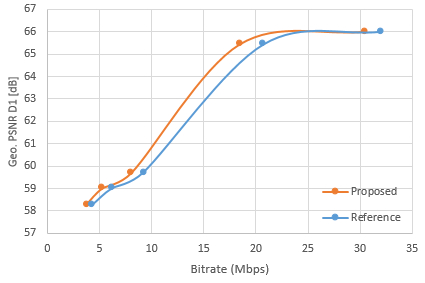
\includegraphics[scale=0.45]{AI_D1_loot_Smooth1_Refine0.png}}%
%	\subfigure[]{%
%		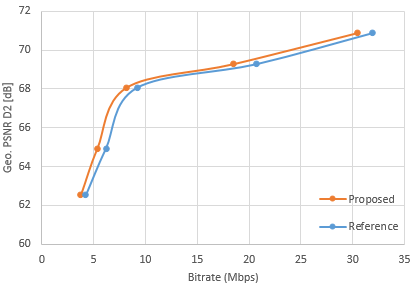
\includegraphics[scale=0.45]{AI_D2_loot_Smooth1_Refine0.png}}%
%	\subfigure[]{%
%		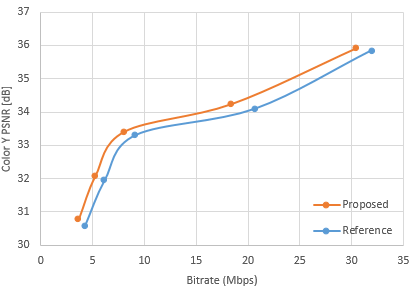
\includegraphics[scale=0.45]{AI_Y_loot_Smooth1_Refine0.png}}%
%	\caption{Rate-Distortion curves for the Loot sequence compared to reference for AI configuration and applying edge smoothing. D1 point-to-point (a), D2 point-to-plane (b), and luma(Y) PSNRs (c)}
%\end{figure}
\begin{figure}[t]
	\centering
	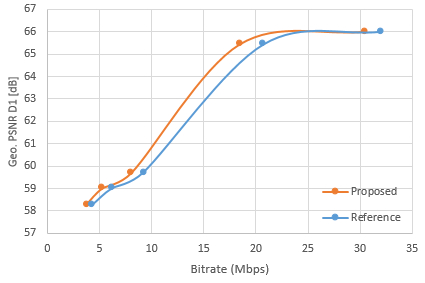
\includegraphics[width=13cm,height=7cm,keepaspectratio]{AI_D1_loot_Smooth1_Refine0.png}\\
	\textsf{(a)}\\
	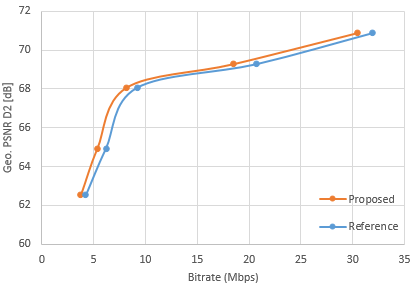
\includegraphics[width=13cm,height=7cm,keepaspectratio] {AI_D2_loot_Smooth1_Refine0.png}\\
	\textsf{(b)}\\
	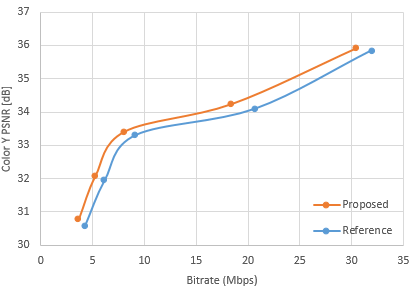
\includegraphics[width=13cm,height=7cm,keepaspectratio]{AI_Y_loot_Smooth1_Refine0.png}\\
	\textsf{(c)}\\
	\caption[]{Rate-Distortion curves for the \textit{Loot} sequence compared to reference for AI configuration and applying edge smoothing. (a) D1 point-to-point , (b) D2 point-to-plane, and (c) luma(Y) PSNRs}
	\label{fig:AI_edge_smoothing}
\end{figure}
\textbf{Random Access Coding Results}\\
\begin{table}
	\centering
	\caption{BD-Rate (\%) and BD-PSNR [dB] performances for Inter-frame and applying Edge-smoothing}
	\label{Inter_frame_Edgesmoothing}
	\scalebox{0.80}{
		\begin{tabular}{|c|c|c|c|c|c|c|c|c|c|c|}
			\hline
			\multirow{2}{*}{Sequence} & \multicolumn{5}{c|}{BD-Rate (\%)} & \multicolumn{5}{c|}{BD-PSNR [dB]}\\
			\cline{2-11}
			& \multicolumn{1}{c|}{D1} & \multicolumn{1}{c|}{D2}& \multicolumn{1}{c|}{Y} & \multicolumn{1}{c|}{U} & \multicolumn{1}{c|}{V}& \multicolumn{1}{c|}{D1} & \multicolumn{1}{c|}{D2}& \multicolumn{1}{c|}{Y} & \multicolumn{1}{c|}{U} & \multicolumn{1}{c|}{V} \\
			\hline
			Loot	    & -18.4\%	& -18.2\%	& -18.8\% &	-35.1\%	& -39.0\% &	1.47 &	1.73 &	0.85 &	1.10 &	1.28 \\
			Redandblack	& -9.1\%	& -9.1\%	& -15.3\% &	-22.7\%	& -14.6\% &	0.64 &	0.75 &	0.80 &	0.56 &	0.54 \\
			Soldier	    &-24.0\%	& -23.4\%	& -26.2\% &	-29.5\%	& -32.0\% &	1.32 &	1.67 &	1.00 &	0.68 &	0.99 \\
			Longdress	&-19.3\%	& -19.2\%	& -22.3\% &	-24.8\%	& -21.8\% &	1.21 &	1.41 &	0.76 &	0.50 &	0.62 \\
			\hline
			\textbf{Average}       & \textbf{-17.7\%} & \textbf{-17.5\%} & 	\textbf{-20.6\%} &	\textbf{-28.0\%} &	\textbf{-26.9\%} &	\textbf{1.16} &	\textbf{1.39} &	\textbf{0.85} & \textbf{0.71} &	\textbf{0.86} \\
			\hline
	\end{tabular}}
\end{table}
%\begin{figure}
%	\centering
%	\subfigure[]{%
%		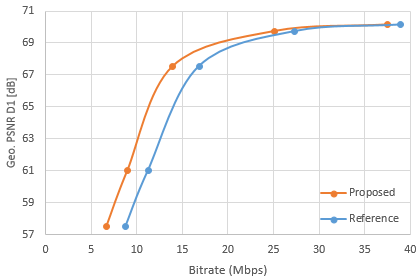
\includegraphics[scale=0.45]{RA_D1_loot_Smooth1_Refine0.png}}%
%	\subfigure[]{%
%		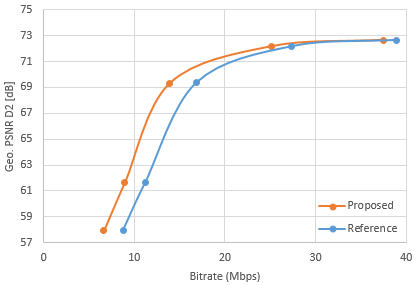
\includegraphics[scale=0.45]{RA_D2_loot_Smooth1_Refine0.png}}%
%	\subfigure[]{%
%		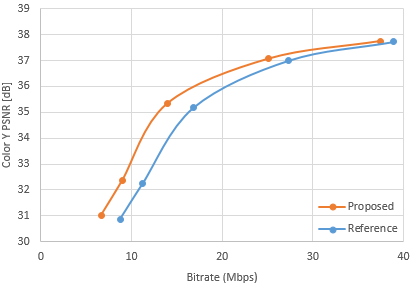
\includegraphics[scale=0.45]{RA_Y_loot_Smooth1_Refine0.png}}%
%	\caption{Rate-Distortion curves for the Loot sequence compared to reference for RA configuration and applying edge smoothing. D1 point-to-point (a), D2 point-to-plane (b), and luma(Y) PSNRs (c)}
%\end{figure}
\begin{figure}[t]
	\centering
	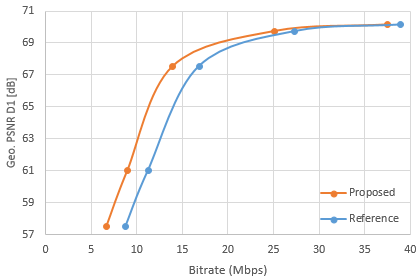
\includegraphics[width=13cm,height=7cm,keepaspectratio]{RA_D1_loot_Smooth1_Refine0.png}\\
	\textsf{(a)}\\
	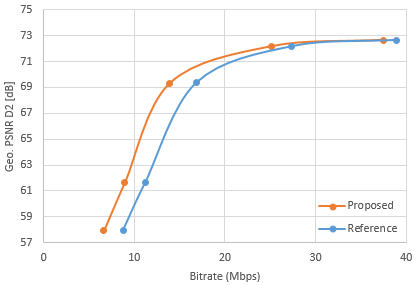
\includegraphics[width=13cm,height=7cm,keepaspectratio] {RA_D2_loot_Smooth1_Refine0.png}\\
	\textsf{(b)}\\
	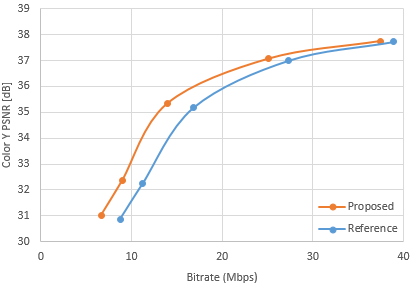
\includegraphics[width=13cm,height=7cm,keepaspectratio]{RA_Y_loot_Smooth1_Refine0.png}\\
	\textsf{(c)}\\
	\caption[]{Rate-Distortion curves for the \textit{Loot} sequence compared to reference for RA configuration and applying edge smoothing. (a) D1 point-to-point , (b) D2 point-to-plane, and (c) luma(Y) PSNRs}
	\label{fig:RA_edge_smoothing}
\end{figure}
\section{Applying Patch refinement}\label{Applying_Patch_refinement_result}
\textbf{All Intra Coding Results}\\
\begin{table}
	\centering
	\caption{BD-Rate (\%) and BD-PSNR [dB] performances for Intra-frame and applying Patch refinement}
	\label{Intra_frame_Patchrefinement}
	\scalebox{0.85}{
		\begin{tabular}{|c|c|c|c|c|c|c|c|c|c|c|}
			\hline
			\multirow{2}{*}{Sequence} & \multicolumn{5}{c|}{BD-Rate (\%)} & \multicolumn{5}{c|}{BD-PSNR [dB]}\\
			\cline{2-11}
			& \multicolumn{1}{c|}{D1} & \multicolumn{1}{c|}{D2}& \multicolumn{1}{c|}{Y} & \multicolumn{1}{c|}{U} & \multicolumn{1}{c|}{V}& \multicolumn{1}{c|}{D1} & \multicolumn{1}{c|}{D2}& \multicolumn{1}{c|}{Y} & \multicolumn{1}{c|}{U} & \multicolumn{1}{c|}{V} \\
			\hline
			Loot           & -3.6\%	& -2.4\% &	-3.2\% &	-2.5\% &	-3.0\% &	0.15 &	0.09 &	0.08 &	0.03 & 	0.05  \\
			Redandblack    & -3.3\%	& -2.2\% &	-2.4\% &	-2.1\% &	-1.9\% &	0.15 &	0.11 &	0.06 &	0.02 &	0.02  \\
			Soldier        & -4.1\%	& -2.8\% &	-3.0\% &	81.0\% &	-2.6\% &	0.16 &	0.13 &	0.07 &	0.03 &	0.03  \\
			Longdress      & -6.1\%	& -5.4\% &	-6.1\% &	-5.3\% &	-5.6\% &	0.27 &	0.27 &	0.12 &	0.02 &	0.07  \\
			\hline
			\textbf{Average}       & \textbf{-4.3\%} & \textbf{-3.2\%} & 	\textbf{-3.7\%} &	\textbf{17.8\%} &	\textbf{-3.3\%} &	\textbf{0.18} &	\textbf{0.15} &	\textbf{0.08} & \textbf{0.02} &	\textbf{0.04} \\
			\hline
	\end{tabular}}
\end{table}
%\begin{figure}
%	\centering
%	\subfigure[]{%
%		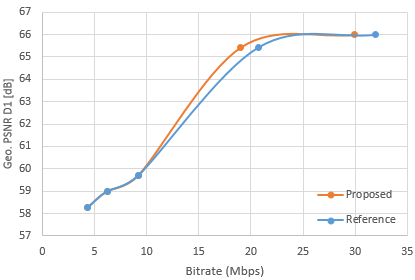
\includegraphics[scale=0.45]{AI_D1_loot_Smooth0_Refine1.png}}%
%	\subfigure[]{%
%		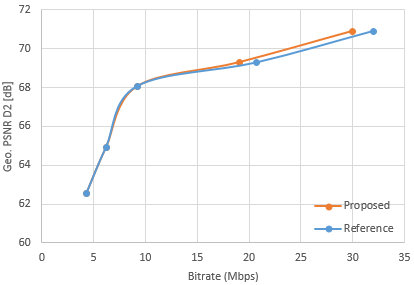
\includegraphics[scale=0.45]{AI_D2_loot_Smooth0_Refine1.png}}%
%	\subfigure[]{%
%		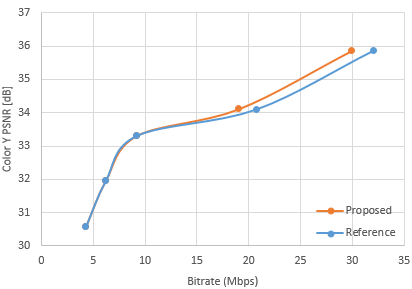
\includegraphics[scale=0.45]{AI_Y_loot_Smooth0_Refine1.png}}%
%	\caption{Rate-Distortion curves for the Loot sequence compared to reference for AI configuration and applying patch refinement. D1 point-to-point (a), D2 point-to-plane (b), and luma(Y) PSNRs (c)}
%\end{figure}
\begin{figure}[t]
	\centering
	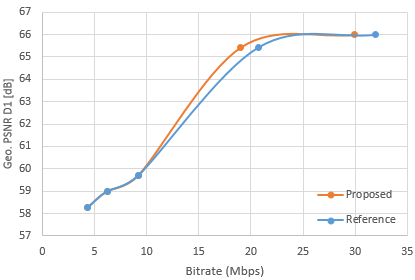
\includegraphics[width=13cm,height=7cm,keepaspectratio]{AI_D1_loot_Smooth0_Refine1.png}\\
	\textsf{(a)}\\
	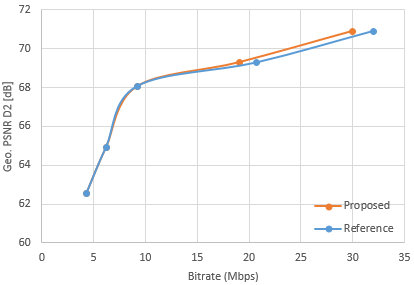
\includegraphics[width=13cm,height=7cm,keepaspectratio] {AI_D2_loot_Smooth0_Refine1.png}\\
	\textsf{(b)}\\
	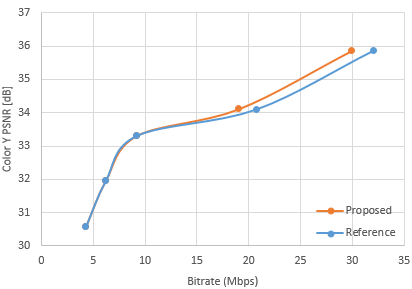
\includegraphics[width=13cm,height=7cm,keepaspectratio]{AI_Y_loot_Smooth0_Refine1.png}\\
	\textsf{(c)}\\
	\caption[]{Rate-Distortion curves for the \textit{Loot} sequence compared to reference for AI configuration and applying patch refinement. (a) D1 point-to-point , (b) D2 point-to-plane, and (c) luma(Y) PSNRs}
	\label{fig:AI_patch_refinement}
\end{figure}
\textbf{Random Access Coding Results}\\
\begin{table}
	\centering
	\caption{BD-Rate (\%) and BD-PSNR [dB] performances for Inter-frame and applying Patch refinement}
	\label{Inter_frame_Patchrefinement}
	\scalebox{0.80}{
		\begin{tabular}{|c|c|c|c|c|c|c|c|c|c|c|}
			\hline
			\multirow{2}{*}{Sequence} & \multicolumn{5}{c|}{BD-Rate (\%)} & \multicolumn{5}{c|}{BD-PSNR [dB]}\\
			\cline{2-11}
			& \multicolumn{1}{c|}{D1} & \multicolumn{1}{c|}{D2}& \multicolumn{1}{c|}{Y} & \multicolumn{1}{c|}{U} & \multicolumn{1}{c|}{V}& \multicolumn{1}{c|}{D1} & \multicolumn{1}{c|}{D2}& \multicolumn{1}{c|}{Y} & \multicolumn{1}{c|}{U} & \multicolumn{1}{c|}{V} \\
			\hline
			Loot	    & -12.9\%	& -12.8\%	& -12.1\%	& -13.2\%	& -13.0\%	& 1.11 &	1.29 &	0.58 &	0.31 &	0.34 \\
			Redandblack	& -9.1\%	& -9.1\%	& -9.5\%	& -9.6\%	& -9.2\%	& 0.63 &	0.74 &	0.49 &	0.21 &	0.32 \\
			Soldier	    & -10.4\%	& -10.4\%	& -10.1\%	& -9.6\%	& -9.5\%	& 0.55 &	0.71 &	0.37 &	0.20 &	0.27 \\
			Longdress	& -11.4\%	& -11.3\%	& -10.8\%	& -11.1\%	& -10.2\%	& 0.67 &	0.77 &	0.35 &	0.19 &	0.27 \\
			\hline
			\textbf{Average}       & \textbf{-11.0\%} & \textbf{-10.9\%} & 	\textbf{-10.6\%} &	\textbf{-10.9\%} &	\textbf{-10.5\%} &	\textbf{0.74} &	\textbf{0.88} &	\textbf{0.45} & \textbf{0.23} &	\textbf{0.30} \\
			\hline
	\end{tabular}}
\end{table}
%\begin{figure}
%	\centering
%	\subfigure[]{%
%		\includegraphics[scale=0.45]{RA_D1_loot_Smooth0_Refine1.png}}%
%	\subfigure[]{%
%		\includegraphics[scale=0.45]{RA_D2_loot_Smooth0_Refine1.png}}%
%	\subfigure[]{%
%		\includegraphics[scale=0.45]{RA_Y_loot_Smooth0_Refine1.png}}%
%	\caption{Rate-Distortion curves for the Loot sequence compared to reference for RA configuration and applying patch refinement. D1 point-to-point (a), D2 point-to-plane (b), and luma(Y) PSNRs (c)}
%\end{figure}
\begin{figure}[t]
	\centering
	\includegraphics[width=13cm,height=7cm,keepaspectratio]{RA_D1_loot_Smooth0_Refine1.png}\\
	\textsf{(a)}\\
	\includegraphics[width=13cm,height=7cm,keepaspectratio] {RA_D2_loot_Smooth0_Refine1.png}\\
	\textsf{(b)}\\
	\includegraphics[width=13cm,height=7cm,keepaspectratio]{RA_Y_loot_Smooth0_Refine1.png}\\
	\textsf{(c)}\\
	\caption[]{Rate-Distortion curves for the \textit{Loot} sequence compared to reference for RA configuration and applying patch refinement. (a) D1 point-to-point , (b) D2 point-to-plane, and (c) luma(Y) PSNRs}
	\label{fig:RA_patch_refinement}
\end{figure}
\section{Applying Edge-smoothing and patch refinement} \label{Applying_edge-smoothing_and_patch_refinement}
\textbf{All Intra Coding Results}\\
\begin{table}
	\centering
	\caption{BD-Rate (\%) and BD-PSNR [dB] performances for Intra-frame and applying both Edge-smoothing and Patch refinement}
	\label{Intra_frame_Edgesmoothing_Patchrefinement}
	\scalebox{0.80}{
		\begin{tabular}{|c|c|c|c|c|c|c|c|c|c|c|}
			\hline
			\multirow{2}{*}{Sequence} & \multicolumn{5}{c|}{BD-Rate (\%)} & \multicolumn{5}{c|}{BD-PSNR [dB]}\\
			\cline{2-11}
			& \multicolumn{1}{c|}{D1} & \multicolumn{1}{c|}{D2}& \multicolumn{1}{c|}{Y} & \multicolumn{1}{c|}{U} & \multicolumn{1}{c|}{V}& \multicolumn{1}{c|}{D1} & \multicolumn{1}{c|}{D2}& \multicolumn{1}{c|}{Y} & \multicolumn{1}{c|}{U} & \multicolumn{1}{c|}{V} \\
			\hline
			Loot	    & -15.0\%	& -14.5\% &	-18.6\%	& -45.8\% &	-41.9\% &	0.65 &	0.64 &	0.52 &	0.75 &	0.85 \\
			Redandblack	& -13.1\%	& -11.6\% &	-15.5\%	& -37.5\% &	-18.7\% &	0.63 &	0.63 &	0.40 &	0.37 &	0.24 \\
			Soldier	    & -18.4\%	& -16.0\% &	-20.0\%	& -92.9\% &	-40.7\% &	0.84 &	0.76 &	0.48 &	0.29 &	0.44 \\
			Longdress	& -20.5\%	& -18.4\% &	-21.8\%	& -32.9\% &	-23.2\% &	0.99 &	0.98 &	0.45 &	0.16 &	0.30 \\
			\hline
			\textbf{Average}       & \textbf{-16.8\%} & \textbf{-15.1\%} & 	\textbf{-19.0\%} &	\textbf{-52.3\%} &	\textbf{-31.1\%} &	\textbf{0.78} &	\textbf{0.75} &	\textbf{0.46} & \textbf{0.39} &	\textbf{0.45} \\
			\hline
	\end{tabular}}
\end{table}
%\begin{figure}
%	\centering
%	\subfigure[]{%
%		\includegraphics[scale=0.45]{AI_D1_loot_Smooth1_Refine1.png}}%
%	\subfigure[]{%
%		\includegraphics[scale=0.45]{AI_D2_loot_Smooth1_Refine1.png}}%
%	\subfigure[]{%
%		\includegraphics[scale=0.45]{AI_Y_loot_Smooth1_Refine1.png}}%
%	\caption{Rate-Distortion curves for the Loot sequence compared to reference for AI configuration and applying edge smoothing patch refinement. D1 point-to-point (a), D2 point-to-plane (b), and luma(Y) PSNRs (c)}
%\end{figure}
\begin{figure}[t]
	\centering
	\includegraphics[width=13cm,height=7cm,keepaspectratio]{AI_D1_loot_Smooth1_Refine1.png}\\
	\textsf{(a)}\\
	\includegraphics[width=13cm,height=7cm,keepaspectratio] {AI_D2_loot_Smooth1_Refine1.png}\\
	\textsf{(b)}\\
	\includegraphics[width=13cm,height=7cm,keepaspectratio]{AI_Y_loot_Smooth1_Refine1.png}\\
	\textsf{(c)}\\
	\caption[]{Rate-Distortion curves for the \textit{Loot} sequence compared to reference for AI configuration and applying edge smoothing patch refinement. (a) D1 point-to-point , (b) D2 point-to-plane, and (c) luma(Y) PSNRs}
	\label{fig:AI_edge_smoothing_patch_refinement}
\end{figure}
\textbf{Random Access Coding Results}\\
\begin{table}
	\centering
	\caption{BD-Rate (\%) and BD-PSNR [dB] performances for Intra-frame and applying both Edge-smoothing and Patch refinement}
	\label{Inter_frame_Edgesmoothing_Patchrefinement}
	\scalebox{0.80}{
		\begin{tabular}{|c|c|c|c|c|c|c|c|c|c|c|}
			\hline
			\multirow{2}{*}{Sequence} & \multicolumn{5}{c|}{BD-Rate (\%)} & \multicolumn{5}{c|}{BD-PSNR [dB]}\\
			\cline{2-11}
			& \multicolumn{1}{c|}{D1} & \multicolumn{1}{c|}{D2}& \multicolumn{1}{c|}{Y} & \multicolumn{1}{c|}{U} & \multicolumn{1}{c|}{V}& \multicolumn{1}{c|}{D1} & \multicolumn{1}{c|}{D2}& \multicolumn{1}{c|}{Y} & \multicolumn{1}{c|}{U} & \multicolumn{1}{c|}{V} \\
			\hline
			Loot          & -29.5\% & -29.3\% & 	-29.2\% &	-43.9\% &	-47.4\% &	2.36 &	2.79 &	1.35 & 1.39 &	1.61 \\
			Redandblack   & -17.5\% & -17.5\% & 	-23.3\% &	-29.8\% &	-22.5\% &	1.30 &  1.53 &	1.26 & 0.78 &	0.87 \\
			Soldier       & -31.4\% & -31.0\% & 	-33.1\% &	-35.9\% &	-37.7\% &	1.79 &	2.30 &  1.31 & 0.86 &	1.21 \\
			Longdress     & -27.6\% & -27.5\% & 	-29.6\% &	-32.0\% &	-28.9\% &	1.77 &	2.08 &	1.03 & 0.67 &	0.85 \\
			\hline
			\textbf{Average}       & \textbf{-26.5\%} & \textbf{-26.3\%} & 	\textbf{-28.8\%} &	\textbf{-35.4\%} &	\textbf{-34.1\%} &	\textbf{1.81} &	\textbf{2.17} &	\textbf{1.24} & \textbf{0.92} &	\textbf{1.14} \\
			\hline
	\end{tabular}}
\end{table}
%\begin{figure}
%	\centering
%	\subfigure[]{%
%		\includegraphics[scale=0.45]{RA_D1_loot_Smooth1_Refine1.png}}%
%	\subfigure[]{%
%		\includegraphics[scale=0.45]{RA_D2_loot_Smooth1_Refine1.png}}%
%	\subfigure[]{%
%		\includegraphics[scale=0.45]{RA_Y_loot_Smooth1_Refine1.png}}%
%	\caption{Rate-Distortion curves for the Loot sequence compared to reference for RA configuration and applying edge smoothing patch refinement. D1 point-to-point (a), D2 point-to-plane (b), and luma(Y) PSNRs (c)}
%\end{figure}
\begin{figure}[t]
	\centering
	\includegraphics[width=13cm,height=7cm,keepaspectratio]{RA_D1_loot_Smooth1_Refine1.png}\\
	\textsf{(a)}\\
	\includegraphics[width=13cm,height=7cm,keepaspectratio] {RA_D2_loot_Smooth1_Refine1.png}\\
	\textsf{(b)}\\
	\includegraphics[width=13cm,height=7cm,keepaspectratio]{RA_Y_loot_Smooth1_Refine1.png}\\
	\textsf{(c)}\\
	\caption[]{Rate-Distortion curves for the \textit{Loot} sequence compared to reference for RA configuration and applying edge smoothing patch refinement. (a) D1 point-to-point , (b) D2 point-to-plane, and (c) luma(Y) PSNRs}
	\label{fig:RA_edge_smoothing_patch_refinement}
\end{figure}
\section{Improved Projection-based Versus the Stat-of-the-art}
\textbf{All Intra Coding Results}\\
\begin{table}
	\centering
	\caption{BD-Rate (\%) and BD-PSNR [dB] performances for Intra-frame comparison Ruf and Seb}
	\label{}
	\scalebox{0.80}{
		\begin{tabular}{|c|c|c|c|c|c|c|c|c|c|c|}
			\hline
			\multirow{2}{*}{Sequence} & \multicolumn{5}{c|}{BD-Rate (\%)} & \multicolumn{5}{c|}{BD-PSNR [dB]}\\
			\cline{2-11}
			& \multicolumn{1}{c|}{D1} & \multicolumn{1}{c|}{D2}& \multicolumn{1}{c|}{Y} & \multicolumn{1}{c|}{U} & \multicolumn{1}{c|}{V}& \multicolumn{1}{c|}{D1} & \multicolumn{1}{c|}{D2}& \multicolumn{1}{c|}{Y} & \multicolumn{1}{c|}{U} & \multicolumn{1}{c|}{V} \\
			\hline
			Loot          & -54.9\%	& -65.9\% &	-59.6\%	& -63.3\% &	-81.0\%	  &   4.41	& 5.06	& 1.92	& 1.42	& 2.83\\
			Redandblack   & -39.0\%	& -48.6\% &	-26.2\%	& -75.0\% &	-100.0\%  & 2.79	& 3.46	& 0.69	& 1.60	& 3.52\\
			Soldier       & -3.0\%	& -56.8\% &	  1.9\%	& -6.6\%	 &   125.9\%  & 0.36	& 4.17	& -0.03	& -0.82	& -1.28\\
			Longdress     & -68.1\%	& -53.8\% &	-56.8\%	& -88.1\% &	-100.0\%  & 5.84	& 4.05	& 1.62	& 1.68	& 3.35\\
			\hline
			\textbf{Average}       & \textbf{-41.2\%} & \textbf{-56.3\%} & 	\textbf{-35.2\%} &	\textbf{-58.3\%} &	\textbf{-38.8\%} &	\textbf{3.35} &	\textbf{4.18} &	\textbf{1.05} & \textbf{0.97} &	\textbf{2.11} \\
			\hline
	\end{tabular}}
\end{table}
%\begin{figure}%
%	\centering
%	\subfigure[]{%
%		\includegraphics[scale=0.4]{AI_D1_loot_Rufael_Seb.png}}%
%	\subfigure[]{%
%		\includegraphics[scale=0.4]{AI_D2_loot_Rufael_Seb.png}}%
%	\subfigure[]{%
%		\includegraphics[scale=0.4]{AI_Y_loot_Rufael_Seb.png}}%
%	\caption{Rate-Distortion curves for the Loot sequence compared to reference for AI configuration and projection-based approach. D1 point-to-point (a), D2 point-to-plane (b), and luma(Y) PSNRs (c)}
%\end{figure}
\begin{figure}[t]
	\centering
	\includegraphics[width=13cm,height=7cm,keepaspectratio]{AI_D1_loot_Rufael_Seb.png}\\
	\textsf{(a)}\\
	\includegraphics[width=13cm,height=7cm,keepaspectratio] {AI_D2_loot_Rufael_Seb.png}\\
	\textsf{(b)}\\
	\includegraphics[width=13cm,height=7cm,keepaspectratio]{AI_Y_loot_Rufael_Seb.png}\\
	\textsf{(c)}\\
	\caption[]{Rate-Distortion curves for the \textit{Loot} sequence compared to reference for AI configuration and projection-based approach. (a) D1 point-to-point , (b) D2 point-to-plane, and (c) luma(Y) PSNRs}
	\label{fig:AI_Rufael_Seb}
\end{figure}

\textbf{Random Access Coding Results}\\
\begin{table}
	\centering
	\caption{BD-Rate (\%) and BD-PSNR [dB] performances for Intra-frame comparison Ruf and Seb}
	\label{}
	\scalebox{0.80}{
		\begin{tabular}{|c|c|c|c|c|c|c|c|c|c|c|}
			\hline
			\multirow{2}{*}{Sequence} & \multicolumn{5}{c|}{BD-Rate (\%)} & \multicolumn{5}{c|}{BD-PSNR [dB]}\\
			\cline{2-11}
			& \multicolumn{1}{c|}{D1} & \multicolumn{1}{c|}{D2}& \multicolumn{1}{c|}{Y} & \multicolumn{1}{c|}{U} & \multicolumn{1}{c|}{V}& \multicolumn{1}{c|}{D1} & \multicolumn{1}{c|}{D2}& \multicolumn{1}{c|}{Y} & \multicolumn{1}{c|}{U} & \multicolumn{1}{c|}{V} \\
			\hline
			Loot          & -71.2\%	& -49.2\%	& -64.8\%	& -84.9\%	& -100.0\%	& 8.08	& 5.51	& 3.50	& 3.76	& 5.22 \\
			Redandblack   & -63.9\%	& -35.1\%	& -17.6\%	& -66.3\%	& -79.3\%	& 5.63	& 3.29	& 0.56	& 2.10	& 4.17
			 \\
			Soldier       & -75.7\%	& -67.2\%	& -58.9\%	& -62.0\%	& -52.3\%	& 6.06	& 6.78	& 2.31	& 1.51	& 1.48
			 \\
			Longdress     & -79.0\%	& -59.5\%	& -65.4\%	& -86.4\%	& -100.0\%	& 8.26	& 5.69	& 2.72	& 3.18	& 4.71
			 \\
			\hline
			\textbf{Average}       & \textbf{-72.4\%}	& \textbf{-52.8\%}	& \textbf{-51.7\%}	& \textbf{-74.9\%}	& \textbf{-82.9\%}	& \textbf{7.01}	& \textbf{5.32}	& \textbf{2.27}	& \textbf{2.64}	& \textbf{3.90}\\
			\hline
	\end{tabular}}
\end{table}
%\begin{figure}
%	\centering
%	\subfigure[]{%
%		\includegraphics[scale=0.4]{RA_D1_loot_Rufael_Seb.png}}%
%	\subfigure[]{%
%		\includegraphics[scale=0.4]{RA_D2_loot_Rufael_Seb.png}}%
%	\subfigure[]{%
%		\includegraphics[scale=0.4]{RA_Y_loot_Rufael_Seb.png}}%
%	\caption{Rate-Distortion curves for the Loot sequence compared to reference for RA configuration and projection-based approach. D1 point-to-point (a), D2 point-to-plane (b), and luma(Y) PSNRs (c)}
%\end{figure}
\begin{figure}[t]
	\centering
	\includegraphics[width=13cm,height=7cm,keepaspectratio]{RA_D1_loot_Rufael_Seb.png}\\
	\textsf{(a)}\\
	\includegraphics[width=13cm,height=7cm,keepaspectratio] {RA_D2_loot_Rufael_Seb.png}\\
	\textsf{(b)}\\
	\includegraphics[width=13cm,height=7cm,keepaspectratio]{RA_Y_loot_Rufael_Seb.png}\\
	\textsf{(c)}\\
	\caption[]{Rate-Distortion curves for the \textit{Loot} sequence compared to reference for RA configuration and applying edge smoothing patch refinement. (a) D1 point-to-point , (b) D2 point-to-plane, and (c) luma(Y) PSNRs}
	\label{fig:RA_Rufael_Seb}
\end{figure}
\begin{figure*}[!tbp]
	\centering
	\subfigure[]{%
		\label{fig:loot_00_32}%
		\includegraphics[scale=0.55]{loot_00_32.png}}%
	\qquad
	\subfigure[]{%
		\label{fig:loot_11_29}%
		\includegraphics[scale=0.55]{loot_11_29.png}}%
	\caption{Decoded point cloud in the 18 Mbit/s for (a) reference, (b) proposed solution}
	\label{fig:comparison_result}
\end{figure*}
Figure \ref{fig:comparison_result} demonstrates the subjective comparison between the reference and proposed methods for the decoded \textit{Loot} sequence in the same bitrate level. As it can be seen from the figure, the proposed solution has improved the quality of the decoded point cloud significantly compared to the reference method.\\

\section{complexity}

\chapter{Conclusion and Future Work} 
what is point cloud? Due to the large number of points which generated to represent the object or scene the limitation for storage and transmission with the current network technology would arise, therefore the necessity of having efficient compression would help this technology to expand in all aspects. The compression can be lossless to lossy.
Projection-based is a novel and efficient method to compress point cloud data. This thesis work highlighted the importance of addressing high frequency content in projection-based compression of volumetric data using 2D video coding technology. Two proposed methods improves the coding efficiency significantly. The proposed algorithms have been implemented and integrated as part of a contribution to the MPEG CfP on Point Cloud Compression \cite{NokiaResponseToCfP} and objective evaluation proves the claim of improvement.\\
%
% The bibliography, i.e the list of references (3 options available)
%
\newpage
\renewcommand{\bibname}{Bibliography}     % Otherwise bilingual babel uses Finnish ``Kirjallisutta''. Strange...
%\renewcommand{\bibname}{L�hteet}         % Set Finnish header, remove this if using English
%\addcontentsline{toc}{chapter}{L�hteet}  % Include this in TOC


%\addcontentsline{toc}{chapter}{\bibname}  % Include this in TOC


%
% Option1: Write the bibliographic information into .bib file
% (e.g. thesis_refs.bib) and use bibtex tool to do the formatting.
%

% You must execute: pdflatex d_tyo.tex; bibtex d_tyo; pdflatex.tex
% First command creates the cross-refeerence file .aux for bibtex and
% last combines the bibtex output to the rest.  Many styles are
% available, see e.g. at
% http://www.ctan.org/tex-archive/biblio/bibtex/base
% http://www.reed.edu/cis/help/latex/bibtexstyles.html


% 1a) Numeric style:
%\bibliographystyle{unsrtnat}
%\bibliographystyle{IEEEtranS}
  
%\bibliographystyle{unsrt}
%\begin{thebibliography}{99}
\bibliography{ref} 

\bibliographystyle{ieeetr}
%\bibliographystyle{unsrt}  % the IEEE's sorted numeric style

 %\end{thebibliography}



\end{document}

